% -*- coding: utf-8 -*-
\chapter{Вычисления и рефлексия}\label{chapter:reflection}

\indexC{eval}
\indexR{вычислитель}
\initial{1.5ex}{2.0ex}{У}{\kern0.5ex никальной чертой} Лиспа является его
вычислитель: \ic{eval}. Хотя в~данной книге вычисления упоминаются чуть~ли
не~на каждой странице, мы никогда не~касались возможности явного использования
вычислителя. И~на то есть веские причины: явные вычисления создают определённые
затруднения с~их формализацией, они влияют на целостность окружения вычислений,
поднимают неудобные вопросы лингвистического плана. Всё это дало жизнь расхожему
выражению: <<\ic{eval}~is~\term{evil}>>. Нахождение возможностей плодотворного
применения \ic{eval} "--- это первый шаг к~рефлексивному программированию "---
теме, которая также будет затронута в~этой главе.

\bigskip

Каждый рассмотренный нами интерпретатор показывал ту или иную сторону процесса
вычислений. Для большинства из них явное предоставление вычислителя
пользователям не~требует значительных усилий и выполняется всего парой строк
кода. Это тривиальная задача по сравнению с~реализацией самого интерпретатора.
Однозначно можно сказать \seePage[basics/sect:evaluation], что облегчение её
решения намеренно заложено в~дизайн Лиспа. Явная функция \ic{eval}
присутствовала ещё в~первых работах отцов"=основателей: \cite{mcc60,mae+62}.

Наличие в~языке явного вычислителя является его фундаментальным качеством,
позволяющим реализовать мощную макросистему, объединить язык и среду разработки,
а также наделить программы уже упомянутыми возможностями интроспекции. Конечно, при этом
имеются и недостатки, такие как макросы, неотрывность среды разработки от~языка
и сующая свой нос куда попало интроспекция. Подобно волшебному джинну, \ic{eval}
может быть как полезной, так и принести погибель.

Итак, какой контракт нам стоит заключить с~\ic{eval}? Безусловно, одним из его
пунктов должно быть утверждение
%
\indexCS{eval}{контракт!идемпотентности}
\begin{equation}\label{reflection/eq:eval-idemp}
  \text{\ic{(eval '$\pi$)}} \eq \pi
\end{equation}
%
Вскоре мы покажем, что это уравнение далеко от однозначности.


\section{Программы и значения}\label{reflection/sect:prog-and-val}

\indexR{вычисления!динамические}
Давайте попробуем добавить \ic{eval} в~самый первый интерпретатор, рассмотренный
в~этой книге. \seePage[basics/sect:basic-evaluator] Он написан на чистом Scheme
без использования каких-либо библиотек. Для начала сделаем \ic{eval} специальной
формой. Следовательно, в~\ic{evaluate} появляется соответствующая ветка:

\indexC{evaluate}
\begin{code:lisp}
(define (evaluate e env)
  (if (atom? e)
      (cond ((symbol? e) (lookup e env))
            ((or (number? e)(string? e)(char? e)
                 (boolean? e)(vector? e) )
              e)
            (else (wrong "Cannot evaluate" e)) )
      (case (car e)
        ((quote) (cadr e))
        ((if)     (if (evaluate (cadr e) env)
                      (evaluate (caddr e) env)
                      (evaluate (cadddr e) env) ))
        ((begin)  (eprogn (cdr e) env))
        ((set!)   (update! (cadr e) env (evaluate (caddr e) env)))
        ((lambda) (make-function (cadr e) (cddr e) env))
        [((eval)   (evaluate (evaluate (cadr e) env) env))]
        (else     (invoke (evaluate (cadr e) env)
                          (evlis (cdr e) env) )) ) ) )
\end{code:lisp}

Специальная форма \ic{eval} вычисляет свой единственный аргумент (прямо как
функция), а затем ещё раз вычисляет полученное в~результате значение в~текущем
окружении. К~сожалению, в~этом вроде как самоочевидном описании на самом деле
полно неясностей.

\indexR{программы!как данные}
\indexR{значения!как программы}
Как уже не~раз было сказано, \ic{evaluate} разделяется на этап анализа и~этап
исполнения. В~последних интерпретаторах мы даже явно ввели две отдельные
функции: \ic{meaning} и \ic{run}. Функция \ic{evaluate} принимает программы, а
возвращает значения "--- результаты вычислений. Вот здесь и возникает первая
проблема (назовём её проблемой типизации): в~форме \ic{(evaluate (evaluate~...)
...)} внешняя \ic{evaluate} применяется к~значению, а не~к~программе.
Являются~ли программы значениями? А~значения программами?

\indexE{Scheme!грамматика}
\indexR{грамматика!Scheme}
Определения языков программирования обычно включают в~себя грамматику "---
описание допустимых синтаксических конструкций этого языка. Грамматика Scheme
приведена в~\cite{kcr98}. Там написано, что определённые наборы букв и скобочек
являются синтаксически допустимыми программами. Кроме того, грамматика задаёт
синтаксис значений (данных), поэтому можно легко проверить, является~ли
программа значением с~синтаксической точки зрения. Благо, в~Scheme есть
универсальная функция \ic{read}, умеющая читать как программы, так и данные.
Ведь ничто не~обязывает нас сразу~же исполнять считанные \ic{read} программы.
Многие интерпретаторы Smalltalk, вроде \cite{gr83}, сперва проверяют синтаксис
программы и отображают её в~специальном окне, подсвечивая все найденные
синтаксические ошибки. Это достаточно распространённая практика, так что при
необходимости вполне можно трактовать программы как значения, если с~точки
зрения синтаксиса они являются нормальными значениями.

Но вот обратное не~всегда верно: существует множество значений, не~являющихся
синтаксически корректными программами, например, \ic{(quote~.~1)}. А~есть и
значения, которые нельзя однозначно отнести к~той или иной группе.

\begin{itemize}
  \item Возьмём значение, являющееся корректной программой во~всём,
        кроме пары-тройки деталей. Например, \ic{(if~\#t 1 (quote~.~2))}.
        Это программа? Если передать данное выражение определённой ранее
        \ic{eval}, то она вычислит его без особых проблем, так как не~будет
        даже смотреть на \ic{(quote~.~2)}. Но данное выражение нарушает
        правила записи программ на~Scheme.

  \item \indexR{внешнее представление}
        Или, например, значение, возвращаемое формой вроде \ic{`(',car
        '(a~b))}, где первым термом является процитированное значение
        функции \ic{car}. Это программа? В~соответствии с~синтаксисом
        \RnRS, это значение не~является программой, так как у~него нет
        \emph{внешнего представления}: его нельзя непосредственно набрать
        на клавиатуре. Тем не~менее, \ic{eval} опять выполнит такую
        программу без~запинки.

  \item % ## -- чтобы TeX не считал #1 за аргумент команды
        \indexE{##n##@\ic{\#\ii{n}\#}, \ic{\#\ii{n}=}}
        \indexR{рекурсия!синтаксическая}
        Теперь воспользуемся нотацией {\CommonLisp}: пусть \ic{\#1=}
        даёт имя следующему за ним выражению, а \ic{\#1\#} позволяет
        сослаться на выражение с~именем~\ic{1}. Держа это в~голове,
        рассмотрим следующую программу, чьё графическое представление
        показано на рисунке~\ref{reflection/prog-and-val/pic:recusive}.
        %
\begin{code:lisp}
(let ((n 4))
  #1=(if (= n 1) 1
         (* n ((lambda (n) #1#) (- n 1))) ) )
\end{code:lisp}
        %
        Это значение содержит цикл. Можно сказать, это синтаксически
        рекурсивная программа. К~сожалению, синтаксис Scheme запрещает
        подобные трюки. Осталось только объяснить это \ic{eval}, которую
        данный цикл ничуть не~смущает.
\end{itemize}

\begin{figure}\begin{center}
% -*- coding: utf-8 -*-
% Синтаксически рекурсивный факториал
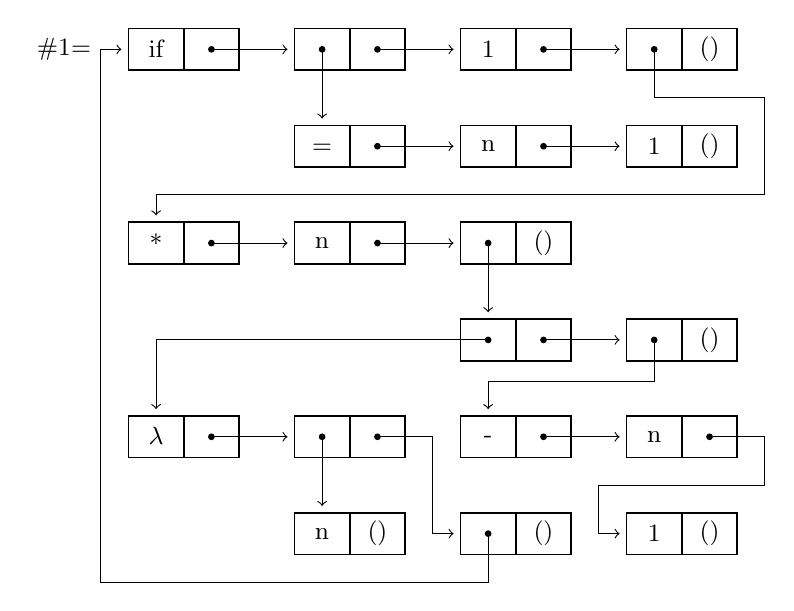
\begin{tikzpicture}
  \tikzstyle{every node}=[font=\small]

% (if ... 1 ...)
  \draw (-1.0em, -0.75em) node[left] {\ic{\#1=}};

  \draw [semithick] ( 0.0em,  0.0em) rectangle  ( 4.0em, -1.5em);
  \draw [semithick] ( 2.0em,  0.0em) -- ( 2.0em, -1.5em);

  \draw [semithick] ( 6.0em,  0.0em) rectangle  (10.0em, -1.5em);
  \draw [semithick] ( 8.0em,  0.0em) -- ( 8.0em, -1.5em);

  \draw [semithick] (12.0em,  0.0em) rectangle  (16.0em, -1.5em);
  \draw [semithick] (14.0em,  0.0em) -- (14.0em, -1.5em);

  \draw [semithick] (18.0em,  0.0em) rectangle  (22.0em, -1.5em);
  \draw [semithick] (20.0em,  0.0em) -- (20.0em, -1.5em);

  \filldraw  ( 3.0em, -0.75em) circle(1.0pt);
  \draw [->] ( 3.0em, -0.75em) -- ( 5.75em, -0.75em);

  \filldraw  ( 9.0em, -0.75em) circle(1.0pt);
  \draw [->] ( 9.0em, -0.75em) -- (11.75em, -0.75em);

  \filldraw  (15.0em, -0.75em) circle(1.0pt);
  \draw [->] (15.0em, -0.75em) -- (17.75em, -0.75em);

  \filldraw  ( 7.0em, -0.75em) circle(1.0pt);
  \draw [->] ( 7.0em, -0.75em) -- ( 7.00em, -3.25em);

  \filldraw  (19.0em, -0.75em) circle(1.0pt);
  \draw [->] (19.0em, -0.75em) -- (19.00em, -2.50em) --
             (23.0em, -2.50em) -- (23.00em, -6.00em) --
             ( 1.0em, -6.00em) -- ( 1.00em, -6.75em);

  \draw ( 1.0em, -0.75em) node {\ic{if}};
  \draw (13.0em, -0.75em) node {\ic{1}};
  \draw (21.0em, -0.75em) node {\ic{()}};

% (= n 1)
  \draw [semithick] ( 6.0em, -3.5em) rectangle  (10.0em, -5.0em);
  \draw [semithick] ( 8.0em, -3.5em) -- ( 8.0em, -5.0em);

  \draw [semithick] (12.0em, -3.5em) rectangle  (16.0em, -5.0em);
  \draw [semithick] (14.0em, -3.5em) -- (14.0em, -5.0em);

  \draw [semithick] (18.0em, -3.5em) rectangle  (22.0em, -5.0em);
  \draw [semithick] (20.0em, -3.5em) -- (20.0em, -5.0em);

  \filldraw  ( 9.0em, -4.25em) circle(1.0pt);
  \draw [->] ( 9.0em, -4.25em) -- (11.75em, -4.25em);

  \filldraw  (15.0em, -4.25em) circle(1.0pt);
  \draw [->] (15.0em, -4.25em) -- (17.75em, -4.25em);

  \draw ( 7.0em, -4.35em) node {\ic{=}};
  \draw (13.0em, -4.25em) node {\ic{n}};
  \draw (19.0em, -4.25em) node {\ic{1}};
  \draw (21.0em, -4.25em) node {\ic{()}};

% (* n ...)
  \draw [semithick] ( 0.0em, -7.0em) rectangle  ( 4.0em, -8.5em);
  \draw [semithick] ( 2.0em, -7.0em) -- ( 2.0em, -8.5em);

  \draw [semithick] ( 6.0em, -7.0em) rectangle  (10.0em, -8.5em);
  \draw [semithick] ( 8.0em, -7.0em) -- ( 8.0em, -8.5em);

  \draw [semithick] (12.0em, -7.0em) rectangle  (16.0em, -8.5em);
  \draw [semithick] (14.0em, -7.0em) -- (14.0em, -8.5em);

  \filldraw  ( 3.0em, -7.75em) circle(1.0pt);
  \draw [->] ( 3.0em, -7.75em) -- ( 5.75em, -7.75em);

  \filldraw  ( 9.0em, -7.75em) circle(1.0pt);
  \draw [->] ( 9.0em, -7.75em) -- (11.75em, -7.75em);

  \filldraw  (13.0em, -7.75em) circle(1.0pt);
  \draw [->] (13.0em, -7.75em) -- (13.00em,-10.25em);

  \draw ( 1.0em, -7.75em) node {\ic{*}};
  \draw ( 7.0em, -7.75em) node {\ic{n}};
  \draw (15.0em, -7.75em) node {\ic{()}};

% (... ...)
  \draw [semithick] (12.0em,-10.5em) rectangle  (16.0em,-12.0em);
  \draw [semithick] (14.0em,-10.5em) -- (14.0em,-12.0em);

  \draw [semithick] (18.0em,-10.5em) rectangle  (22.0em,-12.0em);
  \draw [semithick] (20.0em,-10.5em) -- (20.0em,-12.0em);

  \filldraw  (15.0em, -11.25em) circle(1.0pt);
  \draw [->] (15.0em, -11.25em) -- (17.75em, -11.25em);

  \filldraw  (19.0em, -11.25em) circle(1.0pt);
  \draw [->] (19.0em, -11.25em) -- (19.00em, -12.75em) --
             (13.0em, -12.75em) -- (13.00em, -13.75em);

  \filldraw  (13.0em, -11.25em) circle(1.0pt);
  \draw [->] (13.0em, -11.25em) -- ( 1.00em, -11.25em) -- (1.00em, -13.75em);

  \draw (21.0em, -11.25em) node {\ic{()}};

% (lambda ... #1)   (- n ...)
  \draw [semithick] ( 0.0em,-14.0em) rectangle  ( 4.0em,-15.5em);
  \draw [semithick] ( 2.0em,-14.0em) -- ( 2.0em,-15.5em);

  \draw [semithick] ( 6.0em,-14.0em) rectangle  (10.0em,-15.5em);
  \draw [semithick] ( 8.0em,-14.0em) -- ( 8.0em,-15.5em);

  \draw [semithick] (12.0em,-14.0em) rectangle  (16.0em,-15.5em);
  \draw [semithick] (14.0em,-14.0em) -- (14.0em,-15.5em);

  \draw [semithick] (18.0em,-14.0em) rectangle  (22.0em,-15.5em);
  \draw [semithick] (20.0em,-14.0em) -- (20.0em,-15.5em);

  \filldraw  ( 3.0em, -14.75em) circle(1.0pt);
  \draw [->] ( 3.0em, -14.75em) -- ( 5.75em, -14.75em);

  \filldraw  (15.0em, -14.75em) circle(1.0pt);
  \draw [->] (15.0em, -14.75em) -- (17.75em, -14.75em);

  \filldraw  ( 7.0em, -14.75em) circle(1.0pt);
  \draw [->] ( 7.0em, -14.75em) -- ( 7.00em, -17.25em);

  \filldraw  (21.0em, -14.75em) circle(1.0pt);
  \draw [->] (21.0em, -14.75em) -- (23.00em, -14.75em) --
             (23.0em, -16.50em) -- (17.00em, -16.50em) --
             (17.0em, -18.25em) -- (17.75em, -18.25em);

  \filldraw  ( 9.0em, -14.75em) circle(1.0pt);
  \draw [->] ( 9.0em, -14.75em) -- (11.00em, -14.75em) --
             (11.0em, -18.25em) -- (11.75em, -18.25em);

  \draw ( 1.0em, -14.70em) node {$\lambda$};
  \draw (13.0em, -14.75em) node {\ic{-}};
  \draw (19.0em, -14.75em) node {\ic{n}};

% (n)   (#1#)   (... 1)
  \draw [semithick] ( 6.0em,-17.5em) rectangle  (10.0em,-19.0em);
  \draw [semithick] ( 8.0em,-17.5em) -- ( 8.0em,-19.0em);

  \draw [semithick] (12.0em,-17.5em) rectangle  (16.0em,-19.0em);
  \draw [semithick] (14.0em,-17.5em) -- (14.0em,-19.0em);

  \draw [semithick] (18.0em,-17.5em) rectangle  (22.0em,-19.0em);
  \draw [semithick] (20.0em,-17.5em) -- (20.0em,-19.0em);

  \filldraw  (13.00em, -18.25em) circle(1.0pt);
  \draw [->] (13.00em, -18.25em) -- (13.00em, -20.00em) --
             (-1.00em, -20.00em) -- (-1.00em,  -0.75em) -- (-0.25em, -0.75em);

  \draw ( 7.0em, -18.25em) node {\ic{n}};
  \draw ( 9.0em, -18.25em) node {\ic{()}};
  \draw (15.0em, -18.25em) node {\ic{()}};
  \draw (19.0em, -18.25em) node {\ic{1}};
  \draw (21.0em, -18.25em) node {\ic{()}};
\end{tikzpicture}

\end{center}%
\caption{Синтаксически рекурсивный факториал.}%
\label{reflection/prog-and-val/pic:recusive}
\end{figure}

Конечно, вам может показаться, что все эти примеры взяты из специальной книги
<<Тысяча и одно извращение на Лиспе>>, но зато они вполне доходчиво
демонстрируют, насколько расплывчатой становится идея программы с~появлением
\ic{eval}. Похожие проблемы возникают и у~макросов, проводящих разнообразные
вычисления со~значениями"=программами.

\indexR{ошибки!статические}
\indexR{ошибки!динамические}
\indexR{цитаты!запрещённые}
Кстати, вспомните наш разговор о~статических и динамических ошибках.
\seePage[fast/fast/classify/sssect:static-err] Где именно проводить границу
между ними? Наиболее либеральная позиция: допускать любые синтаксические
аномалии вроде \ic{(quote~. 3)}, пока они не~мешают проводить вычисления.
Наиболее строгая: допускать только такие программы, которые представимы в~виде
конечного ациклического графа синтаксически корректных выражений. В~этом случае
упомянутый ранее синтаксически рекурсивный факториал будет признан недопустимым,
несмотря на то, что отдельные выражения, из которых он состоит, являются вполне
корректными. Пожалуй, мы примем именно эту позицию (её~же занимает и~Scheme),
потому как существует алгоритм, рассмотренный в~\cite{que92a}, позволяющий
переписать произвольную синтаксически рекурсивную программу в~виде дерева
инструкций без~циклов. Что касается цитат, то мы разрешим только цитаты,
состоящие из конечного числа атомов, имеющих внешнее представление. Таким
образом, под запретом цитирования оказываются замыкания, продолжения, порты,
а~также циклические\footnote{Вот именно их можно и разрешить: это не~так сложно
сделать, а они могли~бы быть полезными, например, при реализации \Meroonet.}
конструкции.

\indexR{синтаксис!проверка}
Правила, формализующие понятие синтаксически корректной программы, можно
записать в~виде следующих предикатов. Они проверяют синтаксис выражений и
обнаруживают\footnote{Как думаете, значение \ic{(let ((e~'(x))) `(lambda
,e~,e))} считается допустимой программой?} циклы.

\indexC{program"?}
\indexC{variables-list"?}
\indexC{quotation"?}
\begin{code:lisp}
(define (program? e)
  (define (program? e m)
    (if (atom? e)
        (or (symbol? e) (number? e) (string? e) (char? e) (boolean? e))
        (if (memq e m) #f
            (let ((m (cons e m)))
              (define (all-programs? e+ m+)
                (if (memq e+ m+) #f
                    (let ((m+ (cons e+ m+)))
                      (and (pair? e+)
                           (program? (car e+) m)
                           (or (null? (cdr e+))
                               (all-programs? (cdr e+) m+) ) ) ) ) )
              (case (car e)
                ((quote) (and (pair? (cdr e))
                              (quotation? (cadr e))
                              (null? (cddr e)) ))
                ((if) (and (pair? (cdr e))
                           (program? (cadr e) m)
                           (pair? (cddr e))
                           (program? (caddr e) m)
                           (pair? (cdddr e))
                           (program? (cadddr e) m)
                           (null? (cddddr e)) ))
                ((begin) (all-programs? (cdr e) '()))
                ((set!) (and (pair? (cdr e))
                             (symbol? (cadr e))
                             (pair? (cddr e))
                             (program? (caddr e) m)
                             (null? (cdddr e)) ))
                ((lambda) (and (pair? (cdr e))
                               (variables-list? (cadr e))
                               (all-programs? (cddr e) '()) ))
                (else (all-programs? e '())) ) ) ) ) )
  (program? e '()) )

(define (variables-list? v*)
  (define (variables-list? v* already-seen)
    (or (null? v*)
        (and (symbol? v*)
             (not (memq v* already-seen)) )
        (and (pair? v*)
             (symbol? (car v*))
             (not (memq (car v*) already-seen))
             (variables-list? (cdr v*)
                              (cons (car v*) already-seen) ) ) ) )
  (variables-list? v* '()) )

(define (quotation? e)
  (define (quotation? e m)
    (if (memq e m) #f
        (let ((m (cons e m)))
          (or (null? e) (symbol? e) (number? e)
              (string? e) (char? e) (boolean? e)
              (and (vector? e)
                   (let loop ((i 0))
                     (or (>= i (vector-length e))
                         (and (quotation? (vector-ref e i) m)
                              (loop (+ i 1)) ) ) ) )
              (and (pair? e)
                   (quotation? (car e) m)
                   (quotation? (cdr e) m) ) ) ) ) )
  (quotation? e '()) )
\end{code:lisp}

Вооружившись предикатом \ic{program?}, можно уточнить определение специальной
формы~\ic{eval} следующим образом:

\begin{code:lisp}
... ((eval) (let ((v (evaluate (cadr e) env)))
              (if (program? v)
                  (evaluate v env)
                  (wrong "Illegal program" v) ) )) ...
\end{code:lisp}

\indexR{смысл программ!по отношению к синтаксису}
\indexR{программы!смысл}
\indexR{значения!как программы}
Увы, это определение всё ещё весьма топорно, потому как предыдущие предикаты
не~проверяют, \emph{является~ли} значение программой или корректной цитатой; они
лишь говорят, правильно~ли \emph{записана} программа или цитата. Это предел
информативности, доступной значениям. Значения сами по себе "--- это
ни~программы, ни~цитаты. Действительно, программа "--- это то, что интерпретатор
считает программой, то~же самое касается и цитат. Именно интерпретатор придаёт
смысл значениям. Для уточнения этого момента перейдём к~интерпретатору из
четвёртой главы. \seePage[chapter:assignment] В~нём память и продолжения
используются явно, а значения интерпретируемого Scheme представляются
объектами"=замыканиями. Вот его вычислитель с~добавленной формой~\ic{eval}:

\indexC{evaluate}
\begin{code:lisp}
(define (evaluate e r s k)
  (if (atom? e)
      (if (symbol? e) (evaluate-variable e r s k)
          (evaluate-quote e r s k) )
      (case (car e)
        ((quote)  (evaluate-quote (cadr e) r s k))
        ((if)     (evaluate-if (cadr e) (caddr e) (cadddr e) r s k))
        ((begin)  (evaluate-begin (cdr e) r s k))
        ((set!)   (evaluate-set! (cadr e) (caddr e) r s k))
        ((lambda) (evaluate-lambda (cadr e) (cddr e) r s k))
        [((eval)   (evaluate-eval (cadr e) r s k))]
        (else     (evaluate-application (car e) (cdr e) r s k)) ) ) )

(define (evaluate-eval e r s k)
  (evaluate e r s
    (lambda (v ss)
      (let ((ee (transcode-back v s)))
        (if (program? ee)
            (evaluate ee r ss k)
            (wrong "Illegal program" ee) ) ) ) ) )
\end{code:lisp}

\indexC{load}
\indexC{transcode-back}
В~этом интерпретаторе вычисленное значение первого аргумента формы \ic{eval}
дополнительно преобразуется (с~помощью \ic{transcode-back}) из внутреннего
представления во~внешнее. Затем проверяется правильность записи программы, после
чего она исполняется. Переменные \ic{e} и~\ic{ee} хранят описания программ, а
переменная~\ic{v} "--- значения. Задача \ic{transcode-back}: взять значение и
что"~то с~ним сделать, чтобы его можно было считать корректным описанием
программы. Примерно таким~же путём можно получить \ic{eval} в~интерпретаторе,
где нет \ic{eval}, но есть функция \ic{load}: записываем программу в~файл,
задачу \ic{transcode-back} в~этом случае выполняет \ic{display}; читаем и
исполняем программу из файла с~помощью \ic{load}. Таким образом, программа
<<компилируется>>\footnote{Правда, такой способ определения \ic{eval} позволяет
её использовать только на глобальном уровне, воспользоваться локальным
окружением функций загружаемые программы не~смогут. К~вопросам управления
окружениями при явных вычислениях мы вернёмся чуть позже.} в~имя этого файла.

Наконец, давайте рассмотрим также быстрый интерпретатор из шестой главы.
\seePage[chapter:fast] Там обнаружится ещё несколько интересных моментов. В~нём
значения интерпретируемого языка представляются родными значениями Scheme, так
что нужда в~преобразованиях отпадает. Главной задачей этого интерпретатора было
предварительное вычисление всех выражений, которые можно вычислить статически.

\indexC{meaning}
\indexC{meaning-eval}
\begin{code:lisp}
(define (meaning e r tail?)
  (if (atom? e)
      (if (symbol? e) (meaning-reference e r tail?)
                      (meaning-quotation e r tail?) )
      (case (car e)
        ((quote)  (meaning-quotation (cadr e) r tail?))
        ((lambda) (meaning-abstraction (cadr e) (cddr e) r tail?))
        ((if)     (meaning-alternative (cadr e) (caddr e) (cadddr e)
                                       r tail?))
        ((begin)  (meaning-sequence (cdr e) r tail?))
        ((set!)   (meaning-assignment (cadr e) (caddr e) r tail?))
        [((eval)   (meaning-eval (cadr e) r tail?))]
        (else     (meaning-application (car e) (cdr e) r tail?)) ) ) )

(define (meaning-eval e r tail?)
  (let ((m (meaning e r #f)))
    (lambda ()
      (let ((v (m)))
        (if (program? v)
            (let ((mm (meaning v r tail?)))
              (mm) )
            (wrong "Illegal program" v) ) ) ) ) )
\end{code:lisp}

Вот теперь, на примере компилирующего интерпретатора, преобразующего программы
в~деревья из инструкций-замыканий, становится окончательно понятным, что
компиляция~\ic{v} не~может быть выполнена статически. Впервые узел дерева,
создаваемый компилятором, не~является простой операцией вроде выделения памяти,
проверки условия или обращения к~структурам данных. Вместо этого (о~ужас!)
внутри замыкания находится вызов \ic{meaning}. Это значит, что во~время
исполнения программы требуется держать в~памяти функцию \ic{meaning}, а также
всех её друзей, чтобы иметь возможность выполнять компиляцию программ на~лету,
"--- недешёвое удовольствие!

\bigskip

\indexCS{eval}{параллель с~\ic{quote}}
В~этом разделе мы попытались уменьшить путаницу между понятиями значения и
программы. Похожие отношения существуют также между цитатами и значениями.
Поэтому иногда говорят, что \ic{eval} и~\ic{quote} дополняют друг друга:
\ic{quote} получает описание некоторого значения, которое она должна создать, а
\ic{eval} получает значение, являющееся описанием некоторых действий, которые
она должна выполнить. Важно понимать, что они обе преобразуют обозначения
в~обозначаемые объекты.


\section{\texorpdfstring{\protect\ic{eval} как специальная~форма}%
{eval как специальная форма}}%
\label{reflection/sect:eval-as-spec-form}

\indexR{взаимозаменимость}
\indexCS{eval}{как специальная форма}
\ic{eval} в~виде специальной формы приближает нас к~идеалу "---
уравнению~\eqref{reflection/eq:eval-idemp}; то~есть, \ic{(eval (quote~$\pi$))}
становится эквивалентом~$\pi$. Но это верно лишь при чисто алгебраическом
понимании этого уравнения, как, например, в~\cite{fh89,mul92}. Любая надёжная
теория допускает взаимозаменимость двух объектов только в~случае, когда они
эквивалентны \emph{в~любом контексте}. Точнее говоря, получается, что
\eqref{reflection/eq:eval-idemp} "--- это менее строгая форма
уравнения~\eqref{reflection/eq:eval-idemp-context}, где $C$ означает контекст
вычислений:
%
\indexCS{eval}{контракт!с~контекстом}
\begin{equation}\label{reflection/eq:eval-idemp-context}
  \forall C\colon\ C[\text{\ic{(eval '$\pi$)}}] \eq C[\pi]
\end{equation}

Следовательно, значением замкнутой формы (не~имеющей свободных переменных)
вроде \ic{(eval '((lambda (x~y) x) 1~2))} всегда будет~\ic{1}. Однако,
вычисляемая форма может иметь контекст в~виде лексического окружения:

\begin{code:lisp}
((lambda (x) (eval 'x))
 3 )                       |\is| 3
((lambda (x y) (eval y))
 4 'x )                    |\is| 4
((lambda (x y z) (eval y))
 5 (list 'eval 'z) 'x )    |\is| 5
\end{code:lisp}

\indexR{лексическое окружение!и eval@и~\protect\ic{eval}}
Подобное поведение возможно только при условии, что \ic{eval} доступно
лексическое окружение. В~быстром интерпретаторе замыканию, создаваемому
\ic{meaning} для \ic{eval}, необходимо не~только получить доступ к~функции
\ic{meaning}, но и захватить текущее лексическое окружение~\ic{r} (а~также
\ic{tail?}), чтобы проводить внутренние вычисления в~правильном локальном
лексическом окружении. Следовательно, во~время исполнения программ потребуется
хранить не~только \ic{meaning}, а ещё и всевозможные окружения.

Это видно ещё лучше на примере компилятора в~байт-код из седьмой главы.
\seePage[chapter:compilation] Функция-анализатор \ic{meaning-eval} вызывает
функцию-генератор \ic{EVAL/CE} (от~\term{eval in cur\-rent en\-vi\-ron\-ment}).
Она принимает выражение, которое необходимо вычислить, и окружение для
компиляции.

\indexC{EVAL/CE}
\begin{code:lisp}
(define (meaning-eval e r tail?)
  (let ((m (meaning e r #f)))
    (EVAL/CE m r) ) )

(define (EVAL/CE m r)
  (append (PRESERVE-ENV) (CONSTANT r) (PUSH-VALUE)
          m (COMPILE-RUN) (RESTORE-ENV) ) )
\end{code:lisp}

Функция \ic{EVAL/CE} игнорирует \ic{tail?} и всегда сохраняет локальное
окружение. Новая <<простейшая>> инструкция \ic{COMPILE-RUN} содержит в~себе
весь компилятор"=интерпретатор. Она забирает выражение из регистра \ic{*val*} и
окружение с~верхушки стека, а затем применяет к~ним функцию
\ic{compile-on-the-fly}, которая выполняет компиляцию, загружает в~память
полученный байт-код и передаёт ему управление так, как если~бы там была обычная
функция.

\indexC{COMPILE-RUN}
\indexC{compile-and-run}
\indexC{compile-on-the-fly}
\begin{code:lisp}
(define (COMPILE-RUN) (list 255))

(define-instruction (COMPILE-RUN) 255
  (let ((v *val*)
        (r (stack-pop)) )
    (if (program? v)
        (compile-and-run v r #f)
        (signal-exception #t
          (list "Illegal program" v) ) ) ) )

(define (compile-and-run v r tail?)
  (unless tail? (stack-push *pc*))
  (set! *pc* (compile-on-the-fly v r)) )

(define (compile-on-the-fly v r)
  (set! g.current '())
  (for-each g.current-extend! sg.current.names)
  (set! *quotations* (vector->list *constants*))
  (set! *dynamic-variables* *dynamic-variables*)
  (let ((code (apply vector (append (meaning v r #f) (RETURN)))))
    (set! sg.current.names (map car (reverse g.current)))
    (let ((v (make-vector (length sg.current.names) undefined-value)))
      (vector-copy! sg.current v 0 (vector-length sg.current))
      (set! sg.current v) )
    (set! *constants* (apply vector *quotations*))
    (set! *dynamic-variables* *dynamic-variables*)
    (install-code! code) ) )
\end{code:lisp}

\indexR{компиляция!на лету}
\indexR{загрузчик!динамический}
При компиляции на лету, естественно, потребуются все глобальные переменные,
используемые при обычной компиляции: \ic{g.current} (окружение изменяемых
глобальных переменных), \ic{*quotations*} и \ic{*dynamic-variables*}.%
\footnote*{В~отличие от остальных, переменная \ic{*dynamic-variables*} общая для
компилятора и машины-исполнителя. Сейчас подобные присваивания ей бессмысленны,
но они напоминают, что их необходимо проводить, если данная переменная не~будет
разделяемой.} Откомпилированный код заканчивается инструкцией \ic{RETURN},
возвращающей управление обратно вызывающей программе. После завершения
компиляции окружение исполнения расширяется новыми цитатами, а также глобальными
и динамическими переменными, созданными в~процессе. В~конце концов полученный
фрагмент кода загружается в~память и начинается его исполнение.

\indexCS{eval}{реализация в Си}
\indexR{библиотека!динамически загружаемая}
\indexR{динамически загружаемые библиотеки}
\indexR{сборка мусора!динамическая компиляция}
Подобная загрузка принципиально аналогична механизму динамически подключаемых
библиотек. Для языков вроде~Си \ic{eval} можно свести к~записи строки
с~программой в~файл, компиляции этого файла с~помощью~\ic{cc}, загрузке
средствами операционной системы полученной библиотеки и вызову содержащихся
внутри неё функций. К~сожалению, на данном этапе наша машина не~поддерживает
удаление из памяти загружаемого подобным образом кода, так что он остаётся
висеть мёртвым грузом после завершения исполнения. Мусорить всегда легче, чем
убирать.

Таким образом, стоимость новой специальной формы составляют:

\begin{itemize}
  \item новая инструкция \ic{COMPILE-RUN}, требующая наличия
        функции \ic{meaning} и некоторых другими, что приводит
        к~значительному увеличению размера кода для небольших
        приложений;

  \item расходы памяти на сохранение текущего окружения при каждом
        вызове \ic{eval}.
\end{itemize}

\noindent
К~счастью, дополнительные окружения необходимо сохранять только при этих
вызовах, так что суммарная стоимость использования \ic{eval} линейно зависит
от количества данных форм в~программе.

Кроме того, \ic{eval} иногда используется для отладки: ведь она позволяет
внедрить REPL в~саму программу и просматривать или изменять переменные изнутри,
обращаясь к~ним по именам. А~если туда встроен ещё и отладчик, позволяющий
прервать исполнение программы в~произвольный момент времени (например, по
команде с~клавиатуры), то кроме окружений необходимо вдобавок где"~то хранить и
весь исходный код вместе с~таблицей символов.


\subsection{Глобальные~переменные}%
\label{reflection/eval-as-spec-form/ssect:global}

\indexR{глобальное окружение!и eval@и~\protect\ic{eval}}
Согласно контракту~\eqref{reflection/eq:eval-idemp-context}, выражение \ic{(eval
'(set! foo 33))} должно быть эквивалентным \ic{(set! foo 33)}. Впервые мы
столкнулись с~неоднозначностью семантики присваивания в~четвёртой главе.
\seePage[chapter:assignment] Затем в~разделе~\ref{fast/fast/ssect:variations}
были рассмотрены различные варианты реализации окружений и присваивания.
\seePage[fast/fast/ssect:variations] Следовательно, если для создания переменной
достаточно её упоминания, то и \ic{eval} это позволено. И~наоборот, если
переменные необходимо определять до использования, то данное ограничение
касается в~том числе и~\ic{eval}. Функция \ic{compile-on-the-fly} расширяет
в~конце своей работы глобальное окружение корректно созданными глобальными
переменными компилируемой программы.

\indexCS{eval}{и побочные эффекты}
\indexR{побочные эффекты!и eval@и~\ic{eval}}
Это замечание сделано для того, чтобы вы поняли, что уравнения
\eqref{reflection/eq:eval-idemp} и~\eqref{reflection/eq:eval-idemp-context}
касаются не~только значений $\pi$ и \ic{(eval '$\pi$)}, а и всех иных побочных
эффектов вроде создания новых переменных, изменения значений старых, переходов
{\itd} Именно в~таком смысле надо понимать эквивалентность выражений
в~уравнении~\eqref{reflection/eq:eval-idemp-context}: они должны быть одинаковы
во~всём, везде и всегда. Должно быть абсолютно невозможным\footnote{Это
утверждение носит слегка теоретический характер, так как с~практической точки
зрения можно засечь время выполнения обеих программ. Более медленная, очевидно,
использует~\ic{eval}.} составить программу, которая смогла~бы различить $\pi$
и~\ic{(eval~'$\pi$)} по поведению.


\section{\texorpdfstring{\protect\ic{eval} как функция}{eval как функция}}%
\label{reflection/sect:eval-as-func}

\indexCS{eval}{как примитив}
Специальная форма \ic{eval} вычисляет свой единственный аргумент подобно
функциям, так что возникает логичный вопрос: можно~ли добиться того~же поведения
с~помощью функции, а не~специальной формы? Для ответа на него давайте снова
обратимся к~нашим интерпретаторам и попробуем написать для каждого из них
соответствующий примитив.

С~наивным интерпретатором из первой главы \seePage[basics/sect:basic-evaluator]
всё просто:

\begin{code:lisp}
(defprimitive eval
  (lambda (v)
    (if (program? v)
        (evaluate v env.global)
        (wrong "Illegal program" v) ) ) )
\end{code:lisp}

\indexC{eval/at}
\indexC{eval/ce}
Сразу~же в~глаза бросается один серьёзный момент: \ic{eval} недоступно текущее
лексическое окружение. Так как в~\ic{evaluate} необходимо передать хоть что"~то,
мы берём единственное окружение, которое есть в наличии, "--- глобальное! Следовательно, эта
функция"=вычислитель работает на самом верхнем уровне вложенности "--- уровне
глобальных определений. Назовём её \ic{eval/at}, от~\term{eval at top-level},
а предыдущий вариант будем называть \ic{eval/ce}, если нам потребуется их
различать. Функция \ic{eval/at} не~так~уж и плоха, какой может показаться на
первый взгляд: ей всё~же не~требуется сохранять текущее лексическое окружение,
что экономит немного памяти.

Для пояснения поведения \ic{eval/at} воспользуемся предыдущим примером:

\begin{code:lisp}
(set! x 2) (set! z 1)
((lambda (x) (eval/at 'x))
 3 )                          |\is| 2
((lambda (x y) (eval/at y))
 4 'x )                       |\is| 2
((lambda (x y z) (eval/at y))
 5 (list 'eval/at 'z) 'x )    |\is| 1
\end{code:lisp}

\noindent
При необходимости можно (приближённо) выразить \ic{eval/at} через \ic{eval/ce}:

\begin{code:lisp}
(define (eval/at x) (eval/ce x))
\end{code:lisp}

\noindent
К~сожалению, в~захватываемом \ic{eval/ce} окружении оказывается одна лишняя
переменная "--- локальная переменная~\ic{x} скрывает одноимённую глобальную.
\seeEx[reflection/ex:no-capture] Похоже, эту проблему можно решить, применив
более тонкий подход к~управлению окружениями, поэтому попробуем реализовать
\ic{eval/at} для интерпретатора байт-кодов. Новое определение снова использует
функцию \ic{compile-and-run}, но при этом просит её не~сохранять адрес возврата,
так как он уже был сохранён при вызове функции \ic{eval/at}. Как и в~предыдущем
случае, компиляция выполняется в~единственно доступном окружении \ic{r.init}.

\begin{code:lisp}
(definitial eval
  (let* ((arity 1)
         (arity+1 (+ 1 arity)) )
    (make-primitive
      (lambda ()
        (if (= arity+1 (activation-frame-argument-length *val*))
            (let ((v (activation-frame-argument *val* 0)))
              (if (program? v)
                  (compile-and-run v r.init #t)
                  (signal-exception #t (list "Illegal program" v)) ) )
            (signal-exception #t
              (list "Incorrect arity" 'eval) ) ) ) ) ) )
\end{code:lisp}

Не~стоит понимать ограниченность \ic{eval/at} глобальным уровнем чересчур
буквально, ведь ещё остаются динамические переменные. Совершенно не~важно,
реализована \ic{eval} как специальная форма или функция, "--- следующее
выражение всегда будет работать так, как задумано:

\begin{code:lisp}
(dynamic-let (a 22)
  (eval '(dynamic a)) ) |\is| 22
\end{code:lisp}

Изначальный контракт \ic{eval}, выраженный
уравнением~\eqref{reflection/eq:eval-idemp}, не~подразумевал какого-либо
контекста вообще. Уравнению~\eqref{reflection/eq:eval-idemp-context}, судя по
рассмотренным примерам, \ic{eval/at} тоже не~удовлетворяет. Поэтому для неё мы
составим новый контракт, записанный ниже
в~уравнении~\eqref{reflection/eq:eval-top-context};
здесь переменная~\ii{v} не~захватывается создаваемым замыканием.
%
\indexCS{eval}{контракт!eval/at@\ic{eval/at}}
\begin{equation}\label{reflection/eq:eval-top-context}
  C[\text{\ic{(eval/at '$\pi$)}}] \eq
    \text{\ic{(let ((\ii{v} (lambda () $\pi$)))
      $\displaystyle C[\text{(\ii{v})}]$)}}
\end{equation}

Чаще всего \ic{eval}, реализуемая лисп-системами, является именно \ic{eval/at}.


\section{\texorpdfstring{Цена \protect\ic{eval}}{Цена eval}}%
\label{reflection/sect:cost}

\indexCS{eval}{стоимость}
Довольно сложно оценить суммарную стоимость \ic{eval}. Предположим,
разрабатываемый программный продукт является ничем иным, как \ic{(display
"Hello world!")}. Если специальная форма \ic{eval/ce} не~встречается в~программе
(а~это можно проверить статически), то стоимость её использования нулевая! Если
она всё~же используется, то тянет за собой весь компилятор, так что размер
приложения увеличивается примерно на порядок; скажем, где"~то с~50~килобайт
до~500. Если~же динамический вычислитель реализован в~виде функции и нельзя
доказать, что эта функция не~нужна, то стоимость остаётся примерно той~же.
Код \ic{eval/at} из приложения можно выбросить лишь тогда, когда компилятор
абсолютно уверен в~том, что она никогда не~будет вызвана. Язык может серьёзно
помочь с~доказательством этого утверждения: например, в~Scheme достаточно
убедиться, что глобальная переменная \ic{eval/at} не~упоминается в~программе.
В~{\CommonLisp}, напротив, в~общем случае данное утверждение недоказуемо, так
как кроме всего прочего потребуется доказать, что никто и нигде не~создал строку
\ic{"eval/at"}, не~превратил её в~символ с~помощью \ic{find-symbol} и не~получил
соответствующую функцию с~помощью \ic{symbol-function}. Уже страшно? А~теперь
представьте, что сама \ic{symbol-function} вызывается таким~же образом

А~что насчёт самой \ic{eval}, можно~ли как"~то контролировать значения её
аргумента? Аналогично "--- нет. Это вряд~ли возможно выполнить одновременно
легко, быстро и статически, не~лишив при этом \ic{eval} выразительности, так что
придётся считать, что ей может быть передано любое значение. Следовательно, мы
не~можем трогать ни~одну глобальную переменную вообще, так как \emph{всё}
потенциально может быть использовано и вызвано. Скомпилированное приложение
должно содержать все без исключения возможности языка, что для мощных языков
вроде {\CommonLisp} означает увеличение размеров получаемого приложения ещё на
один порядок.

\indexCS{eval}{и~оптимизации}
И~это ещё далеко не~самое ужасное. Если не~предпринять никаких мер для строгого
контроля над использованием глобального окружения, как в~\cite{qp91b}, где
система модулей позволяет управлять доступом на чтение и модификацию глобальных
переменных, то \ic{eval} убивает на корню многие возможности для оптимизации.
Рассмотрим следующий пример:

\ForLayout{display}{\clearpage}

\begin{code:lisp}
(define (fib n)
  (if (< n 2) (eval (read))
      (+ (fib (- n 1)) (fib (- n 2))) ) )
\end{code:lisp}

Не~будем пока обращать внимание на другие возможные варианты поведения
\ic{eval}, сконцентрируемся на том, что она способна изменить значение
переменной \ic{fib}. Следовательно, при рекурсивном вызове потребуется заново
извлекать адрес функции из глобальной переменной \ic{fib}, а не~просто вслепую
прыгать по \ic{GOTO}. Так как \ic{eval} может изменить любую переменную, нельзя
больше полагаться на привычные методы анализа неизменяемости глобального
окружения. Одно"=единственное обращение к~\ic{eval} может привести к~абсолютно
непредсказуемым последствиям.

По всем перечисленным причинам \ic{eval} считается дорогим удовольствием. Тем
не~менее, в~большом приложении (где кода на несколько мегабайт) и во~время
разработки, когда всё меняется и отбрасывается, \ic{eval} может быть весьма
полезной. Действительно, если понадобится динамически проводить несложные
вычисления, то часто проще и эффективнее (с~точки зрения количества времени,
затраченного на разработку, умноженного на зарплату разработчика) использовать
для этого \ic{eval}, нежели писать и отлаживать с~нуля свой собственный
интерпретатор. Лисп "--- удивительно расширяемый язык, и наличие \ic{eval}
в~стандартной библиотеке "--- это его серьёзное преимущество.


\section{\texorpdfstring{Интерпретируемая \protect\ic{eval}}%
{Интерпретируемая eval}}%
\label{reflection/sect:interpreted-eval}

\indexCS{eval}{интерпретируемая}
\indexR{интерпретатор!встроенный в~язык}
Судя по этой книге, написание интерпретатора Scheme не~представляет особых
трудностей. Допустим, в~лисп-системе нет \ic{eval}, может~ли пользователь
реализовать её самостоятельно? В~конце концов, существует огромный выбор
интерпретаторов, пользователю достаточно скачать понравившийся (или написать
самостоятельно) и включить его в~свою программу, правда? Ну, и~да, и~нет.

Если интерпретатор пишется на Scheme, то это может только функция, так как
в~Scheme нельзя определять новые специальные формы. Кроме того, возникают две
проблемы иного рода.


\subsection{Взаимозаменимость представлений}%
\label{reflection/interpreted-eval/ssect:interchange}

\indexR{протокол вызова функций!при явных вычислениях}
\indexR{взаимозаменимость}
Первая из упомянутых проблем касается взаимодействия между базовым языком и
написанным на нём интерпретатором. Дело в~том, что интерпретатор не~может
вводить новые типы данных, он вынужден пользоваться типами данных, которые ему
предоставляет базовый язык, чтобы программы могли понимать друг друга. Если
интерпретатор пользуется точечными парами, то они должны быть точечными парами
базового языка; логические значения и числа должны быть одними и теми~же;
функции обоих языков должны соблюдать один и тот~же протокол вызова. Результат
любых динамических вычислений должен быть пригоден для использования в~основной
программе, как в~следующем примере:

\begin{code:lisp}
((eval '(lambda (x) (cons x x)))
 33 )    |\is| (33 . 33)
\end{code:lisp}

И~наоборот, интерпретатор тоже должен уметь пользоваться функциями базового
языка:

\begin{code:lisp}
(((eval '(lambda (f)
           (lambda (x) (f x)) ))
  list )
 44 )    |\is| (44)
\end{code:lisp}

Один из вариантов общего протокола вызова: всегда использовать функции
с~произвольной арностью: \ic{(lambda values~...)}, тогда достаточно научить
интерпретатор вынимать аргументы из списков. Для интерпретатора из первой главы,
к~примеру, это делается соответственно его природе "--- элементарно и~наивно:

\indexC{invoke}
\begin{code:lisp}
(define (invoke fn args)
  (if (procedure? fn)
      (apply fn args)
      (wrong "Not a function" fn) ) )

(define (make-function variables body env)
  (lambda values
    (eprogn body (extend env variables values)) ) )
\end{code:lisp}

Кроме того, необходимо позаботиться об~ошибках: внешний интерпретатор должен
уметь понимать и обрабатывать ошибки, возникающие во~внутреннем. Этот вопрос
мы обойдём стороной.


\subsection{Глобальное окружение}%
\label{reflection/interpreted-eval/ssect:global}

\indexR{глобальное окружение!динамическое расширение}
Вторая проблема касается различия представлений глобального окружения. Каждый из
наших интерпретаторов определяет глобальное окружение по-своему, используя
макросы \ic{definitial}, \ic{defprimitive} и~другие. Но теперь интерпретатор
обязан пользоваться глобальным окружением базового языка, или хотя~бы обеспечить
корректную синхронизацию его состояния. Что~бы там ни~было, следующая программа
должна выполняться правильно и без~ошибок:

\begin{code:lisp}
(begin (set! foo 128)
       (eval '(set! bar (+ foo foo)))
       bar )                          |\is| 256
\end{code:lisp}


\subsubsection{Автономные скомпилированные приложения}%
\label{reflection/interpreted-eval/global/sssect:autonomous}

\indexR{глобальное окружение!и eval@и~\protect\ic{eval}!в~автономных приложениях}
\indexR{автономные приложения}
Компиляторы вроде Scheme$\to$C~\cite{bar89} или Bigloo~\cite{ser94} работают
с~файлами, в~которых хранится фиксированный исходный код. Получаемые таким
образом автономные приложения принципиально не~могут пользоваться переменными,
которые не~были явно упомянуты в~исходном коде. Следовательно, переменные,
создаваемые \ic{eval}, будут доступны только внутри \ic{eval}. В~таких условиях
возможно лишь обеспечить интерпретатору доступ к~глобальным переменным внешней
программы. Ответственной за это будет пара функций \ic{global-value} и
\ic{set-global-value!}. Компилятор автоматически формирует эти функции
в~процессе чтения программы. \seeEx[compilation/ex:global-value] По окончании
обработки они будут содержать все используемые\footnote{Конечно~же, переменные
вроде \ic{car} не~включаются в~определение \ic{set-global-value!} для
обеспечения их неизменяемости.} глобальные переменные. Этот список является
статическим, неизменным во~время работы скомпилированного приложения.

\indexC{global-value}
\indexC{set-global-value"!}
\begin{code:lisp}
(define (global-value name)
  (case name
    ((car) car)
    ...
    ((foo) foo)
    (else (wrong "No such global variable" name)) ) )

(define (set-global-value! name value)
  (case name
    ((foo) (set! foo value))
    ...
    (else (wrong "No such mutable global variable" name)) ) )
\end{code:lisp}

Интерпретатор может создавать у~себя внутри столько глобальных переменных,
сколько ему нужно, но ни~одна из них не~будет видна внешней программе. Тем
не~менее, интерпретатор может общаться с~внешней программой посредством тех
переменных, которые существовали в~момент компиляции.


\subsubsection{Интерактивная система}%
\label{reflection/interpreted-eval/global/sssect:interactive}

\indexR{глобальное окружение!и eval@и~\protect\ic{eval}!в~интерактивной сессии}
Если~же работа с~лисп-системой происходит с~помощью REPL, то и~система,
и~интерпретатор могут создавать новые переменные. Приведённая ранее программа
является хорошим примером такого взаимодействия: внешняя система запрашивает
значение переменной, созданной внутренним интерпретатором, который запросил
значение переменной, созданной системой:

\begin{code:lisp}
? (begin (set! foo 128)
         (eval '(set! bar (+ foo foo)))
         2001 )
= 2001
? bar
= 256
\end{code:lisp}

Есть несколько вариантов реализации подобного сотрудничества.


\subsubsection{Символы}%
\label{reflection/interpreted-eval/global/sssect:symbols}

\indexR{символы!связь с~переменными}
Традиционное решение заключается в~использовании символов. Одним из столпов
семантики Лиспа является тесная взаимосвязь понятий символа и~переменной:
переменные записываются с~помощью символов, а символы (как показано далее)
могут играть роль переменных.

\indexC{string->symbol}
\indexR{хеш-таблицы}
Символы "--- это составные структуры данных, имеющие как минимум одно поле:
строку с~собственным именем. В~Scheme символы можно создавать явно с~помощью
функции \ic{string->symbol}. Имена символов уникальны. Обычно это гарантируется
хеш-таблицей, связывающей строки с~символами. Функция \ic{string->symbol}
сначала пытается отыскать строку в~данной хеш-таблице; если такая строка там
есть, то она возвращает соответствующий символ, а в~противном случае
\ic{string->symbol} создаёт новый символ и заносит его в~таблицу на будущее.
Иногда ради ускорения поиска используются различные вспомогательные скрытые
поля, связывающие группы символов между собой.

\indexR{символы!списки свойств}
\indexR{списки свойств}
Часто символы имеют также списки свойств. Обычно они реализуются в~виде
P"~списков, но нередко в~этой роли можно встретить A"~списки или хеш-таблицы. От
выбора внутренней структуры данных зависят потребление памяти и скорость доступа
к~свойствам. Некоторые лисп-системы, например {\LeLisp}, даже хранят в~символах
специальные кеш-поля, служащие для ускорения доступа к~часто используемым
свойствам вроде особенностей форматирования внешнего представления форм,
начинающихся с~данного символа.

\indexR{глобальные переменные!как поля символов}
\indexR{переменные!глобальные}
\indexE{Cval}
\indexE{Fval}
Раз~уж любой символ имеет столько полей, то почему~бы не~добавить туда ещё одно
для хранения значения одноимённой глобальной переменной? В~случае \Lisp2,
конечно, понадобятся два поля: для переменной и для функции. Ничто не~ново под
солнцем, именно так часто и поступают при реализации (например,
\cite{cha80,gp88}), называя эти поля Cval и~Fval. Вдобавок предоставляются
функции для доступа к~этим полям. В~{\CommonLisp} они носят имена
\ic{symbol-value} и~\ic{(setf symbol-value)}, а также \ic{symbol-function}
и~\ic{(setf symbol-function)}.

Такое решение привлекательно своей стопроцентной гарантией правильной работы.
Каждый символ, используемый в~программе, уже был создан \ic{string->symbol},
которую вызвала \ic{read} в~процессе чтения программы. Конечно, не~всякий символ
используется для хранения значения глобальной переменной, но важно, что всякая
глобальная переменная гарантированно имеет соответствующий символ.

Поэтому достаточно предоставить всего две функции: \ic{global-value}
и~\ic{set-global-value!}, позволяющие просматривать и изменять значения
глобальных переменных, ссылаясь на них по именам. Интерпретатор \ic{eval}
сможет воспользоваться глобальными переменными базового языка посредством этих
функций, а проблема корректного расширения глобального окружения пропадает
в~принципе "--- она автомагически решается механизмом доступа к~символам.

Покажем на примере интерпретатора из первой главы, как использовать эти функции.
Окружение \ic{env} теперь будет содержать только локальные переменные, а
глобальные будут использоваться напрямую "--- теперь они совпадают с~глобальными
переменными того Scheme, на котором написан интерпретатор. Таким образом,
получаем:

\indexC{lookup}
\indexC{update"!}
\begin{code:lisp}
(define (lookup id env)
  (if (pair? env)
      (if (eq? id (caar env))
          (cdar env)
          (lookup id (cdr env)) )
      (global-value id) ) )

(define (update! id env value)
  (if (pair? env)
      (if (eq? id (caar env))
          (begin (set-cdr! (car env) value)
                 value )
          (update! id (cdr env) value) )
      (set-global-value! id value) ) )
\end{code:lisp}

\indexCS{global-value}{цена}
\indexCS{set-global-value"!}{цена}
Данное решение кажется элегантным, но эта элегантность приобретается за
внушительную цену: ведь теперь \emph{любая} глобальная переменная доступна по
имени. В~случае автономного приложения \ic{global-value} вынуждает нас включать
в~приложение всю без исключения библиотеку функций, так как любое имя может быть
вычислено, а значит, любая функция может понадобиться. Это не~особо критично для
среды разработки, так как она затем и существует, чтобы абсолютно всё было под
рукой, но вот с~маленькими автономными приложениями такой подход сочетается
плохо. Более того, функция \ic{set-global-value!} может изменить значение любой
изменяемой глобальной переменной, что, конечно~же, оказывает закономерный эффект
на оптимизации компилятора.

\indexC{symeval}
Пару функций \ic{global-value} и \ic{set-global-value!} можно понимать как
специализированную версию \ic{eval} для переменных. Между прочим, в~некоторых
старых лисп-системах так оно и~было: этот специализированный вычислитель
назывался \ic{symeval}. Также можно их считать парой рефлексивных функций,
реифицирующих доступ к~глобальным переменным. Написать <<\ic{foo}>>, чтобы
получить значение глобальной переменной \ic{foo}, "--- это то~же самое, что
неявно вычислить значение формы \ic{(global~'foo)}.


\subsubsection{Полноценные окружения}%
\label{reflection/interpreted-eval/global/sssect:first-class}

Другой вариант решения проблемы окружений состоит в~определении \ic{eval} как
функции двух переменных: выражения, которое необходимо вычислить, и окружения,
в~котором будут проводиться вычисления. Бинарная \ic{eval} наивного
интерпретатора вроде как подходит по сигнатуре, но при этом упускается один
важный момент: аргументом функции может быть только значение. Внутри
интерпретатора окружения просто существуют, не~являясь при этом полноценными
значениями языка. Следовательно, для реализации этой идеи необходимо определить
операцию реификации окружений, превращающую их в~полноценные объекты. Кроме
того, было~бы полезным иметь и другие возможности вроде модификации окружений
или хотя~бы извлечения значений переменных из них. Наличие соответствующих
функций позволяет реализовать механизм взаимодействия окружений интерпретатора
с~окружениями внешней системы. Такой подход поднимает множество специфичных
вопросов, которые мы сейчас и~рассмотрим.


\section{Реификация окружений}\label{reflection/sect:reify-env}

\indexR{контекст вычислений}
\indexR{окружение!как тип данных}
\indexR{окружение!как полноценный объект}
\indexR{полноценные объекты!окружения}
\indexR{полноценные объекты!продолжения}
\indexR{реификация}
Денотационный интерпретатор чётко показал, что контекст вычислений в~Scheme
является тройкой из окружения, продолжения и~памяти. Отложив память в~дальний
угол, сфокусируемся на оставшейся паре. Продолжения уже могут становиться
полноценными объектами языка благодаря \ic{call/cc} или \ic{bind-exit}.
Окружениями~же возможно пользоваться только неявно. В~данном разделе мы
рассмотрим, как превратить их в~объекты, допускающие явную программную
манипуляцию.

\indexR{окружение!операции}
\indexR{захват привязок}
\indexR{привязки (bindings)}
Добиться этого можно различными способами, сохраняющими те или иные свойства,
допускающими те или иные операции. Подробную классификацию можно найти
в~\cite{ra82,mr91}. Существуют три фундаментальные операции над окружениями:
поиск значения переменной, изменение значения переменной и добавление новой
переменной в~окружение. Реификация окружений фактически сводится к~захвату
соответствующих привязок переменных к~значениям. Привязки при этом становятся
явными, что позволяет реализовать вышеприведённые операции как обычные функции
языка.


\subsection{\texorpdfstring{Специальная~форма \protect\ic{export}}%
{Специальная форма export}}%
\label{reflection/reify-env/ssect:export}

\indexR{специальные формы!export@\protect\ic{export}}
\indexC{export}
\indexC{eval/b}
Начнём со~специальной формы, называемой \ic{export}: ей передаётся список имён
переменных, а в~ответ она возвращает окружение с~соответствующими привязками.
Полученное окружение можно будет впоследствии передать вторым аргументом
в~бинарную функцию \ic{eval} (впредь будем называть её \ic{eval/b}). Например:

\ForLayout{display}{\begingroup\lstset{aboveskip=\smallskipamount}}

\begin{code:lisp}
(let ((r (let ((x 3)) (export x))))
  (eval/b 'x r) )                    |\is| 3

(let ((f+r (let ((x 3))
             (cons (lambda () x) (export x)) )))
  (eval/b '(set! x (+ 1 x)) (cdr f+r))
  ((car f+r)) )                      |\is| 4

(let ((r (export car cons)))
  (let ((car cdr))
    (eval/b '(car (cons 1 2)) r) ) ) |\is| 1
\end{code:lisp}

\ForLayout{display}{\endgroup}

Первый пример показывает, что объект-окружение, содержащий привязку
переменной~\ic{x}, действительно создаётся, а \ic{eval/b} это окружение успешно
переваривает. Второй пример демонстрирует изменяемость переменной~\ic{x} и
доказывает, что захватывается действительно привязка, так как иным способом
изменить значение свободной переменной замыкания невозможно. Третий пример
показывает, что можно захватывать и глобальные привязки.

\indexR{окружение!операции!создание}
Специальная форма \ic{export} позволяет жонглировать окружениями по желанию:
захватить окружение в~одном месте, а использовать в~совершенно другом.
Реализация данной формы нетривиальна, так что её стоит рассмотреть подробнее.
Как обычно, начинаем с~добавления новой формы в~синтаксический анализатор
\ic{meaning}:

\begin{code:lisp}
... ((export) (meaning-export (cdr e) r tail?)) ...
\end{code:lisp}

Естественно, захваченное окружение должно содержать не~только список записей
активаций, но также полный перечень имён и адресов переменных. Та~же информация
была нужна \ic{eval/ce}, как вы помните. Поэтому реифицированные окружения будут
представляться объектами с~двумя полями: списком записей активаций и списком пар
<<имя "--- адрес>>, по которому программы смогут разобраться, что где находится.
(См.~рисунок~\ref{reflection/reifiy-env/export/pic:reified-env}.)

\indexC{reified-environment}
\begin{code:lisp}
(define-class reified-environment Object
  ( sr r ) )
\end{code:lisp}

\begin{figure}\begin{center}
% -*- coding: utf-8 -*-
% Представление окружений
\begin{tikzpicture}
  \tikzstyle{every node}=[font=\small]

  \draw (0.0em, 0.1em) node[anchor = south west] {\ii{записи активаций}};

  \draw [semithick] (0.0em,  0.00em) rectangle (4.0em, -3.75em);
  \draw             (0.0em, -1.25em) -- (4.0em, -1.25em);
  \draw [dashed]    (0.0em, -2.50em) -- (4.0em, -2.50em);

  \filldraw  (2.0em, -0.625em) circle(1.0pt);
  \draw [->] (2.0em, -0.625em) -- (7.25em, -0.625em);

  \draw [semithick] (7.5em,  0.00em) rectangle (11.5em, -5.00em);
  \draw             (7.5em, -1.25em) -- (11.5em, -1.25em);
  \draw [dashed]    (7.5em, -2.50em) -- (11.5em, -2.50em);
  \draw [dashed]    (7.5em, -3.75em) -- (11.5em, -3.75em);

  \filldraw  (9.5em, -0.625em) circle(1.0pt);
  \draw [->] (9.5em, -0.625em) -- (13.50em, -0.625em);

  \draw (13.3em, -0.55em) node[right] {\ii{nil}};



  \draw (20.50em, 0.1em) node[above] {\ii{глобальное окружение}};

  \draw [semithick] (19.5em,  0.0em) rectangle (23.5em, -10.0em);
  \draw             (19.5em, -4.0em)  -- (23.5em, -4.0em);
  \draw             (19.5em, -5.25em) -- (23.5em, -5.25em);

  \draw (21.5em, -3.625em) node[above] {$\vdots$};
  \draw (21.5em, -5.125em) node[below] {$\vdots$};

  \draw (23.5em, -4.625em) node[right] {\footnotesize\ic{23}};
  \draw (23.5em, 0.0em) node[anchor = north west] {\footnotesize\ic{0}};



  \draw (-6.5em, 0.1em) node[above, text width = 4.5em, align = left]
          {\ii{реифицированное окружение}};

  \draw [semithick] (-8.0em, 0.0em) rectangle (-5.0em, -2.5em);
  \draw             (-8.0em, -1.25em) -- (-5.0em, -1.25em);

  \filldraw  (-6.5em, -0.625em) circle(1.0pt);
  \draw [->] (-6.5em, -0.625em) -- (-0.25em, -0.625em);

  \filldraw  (-6.5em, -1.875em) circle(1.0pt);
  \draw [->] (-6.5em, -1.875em) -- (-6.5em, -6.5em);

  \draw (-8.5em, -6.0em) node[rectangle, anchor = north west] {%
\begin{code:lisp}
( (foo (local 0 0))
  (bar (local 1 2))
  (hux (global 23))
  ... )
\end{code:lisp}};

  \draw [dashed, ->] (-3.0em, -6.75em) --
                     (-3.0em, -1.875em) -- (-0.25em, -1.875em);
  
  \draw [dashed, ->] (1.25em, -8.375em) -- (5.25em, -8.375em) --
                     (5.25em, -4.375em) -- (7.25em, -4.375em);
  
  \draw [dashed, ->] (1.25em, -9.5em) -- (15.50em, -9.5em) --
                     (15.50em, -4.625em) -- (19.25em, -4.625em);

\end{tikzpicture}

\end{center}%
\caption{Представление окружений.}%
\label{reflection/reifiy-env/export/pic:reified-env}%
\end{figure}

Не~особо (пока) углубляясь в~детали, будем компилировать форму \ic{export}
следующим образом:

\indexC{meaning-export}
\indexC{CREATE-1ST-CLASS-ENV}
\indexC{create-first-class-environment}
\begin{code:lisp}
(define (meaning-export n* r tail?)
  (unless (every? symbol? n*)
          (static-wrong "Incorrect variables" n*) )
  (append (CONSTANT (extract-addresses n* r)) (CREATE-1ST-CLASS-ENV)) )

(define (CREATE-1ST-CLASS-ENV) (list 254))

(define-instruction (CREATE-1ST-CLASS-ENV) 254
  (create-first-class-environment *val* *env*) )

(define (create-first-class-environment r sr)
  (set! *val* (make-reified-environment sr r)) )
\end{code:lisp}

Список пар <<имя "--- адрес>> передаётся как цитата через регистр \ic{*val*},
его оттуда забирает новая инструкция \ic{CREATE-1ST-CLASS-ENV}, которая создаст
соответствующий объект.

\indexR{представление!лексических окружений}
\indexR{лексическое окружение}
Для упрощения вычислений мы немного изменим представление статической части
окружений (значений переменной~\ic{r}). Вместо <<гирлянд>> они теперь будут
просто ассоциативными списками, как на
рисунке~\ref{reflection/reifiy-env/export/pic:reified-env}. Это небольшое
изменение, но упрощение \ic{compute-kind} приобретается ценой усложнения
\ic{r-extend*}: теперь при каждом расширении окружения необходимо переносить
уже существующие переменные на один уровень глубже.

\indexC{compute-kind}
\indexC{r-extend*}
\indexC{bury-r}
\begin{code:lisp}
(define (compute-kind r n)
  (or (let ((var (assq n r)))
        (and (pair? var) (cadr var)) )
      (global-variable? g.current n)
      (global-variable? g.init n)
      (adjoin-global-variable! n) ) )

(define (r-extend* r n*)
  (let ((old-r (bury-r r 1)))
    (let scan ((n* n*) (i 0))
      (cond ((pair? n*) (cons (list (car n*) `(local 0 . ,i))
                              (scan (cdr n*) (+ i 1)) ))
            ((null? n*) old-r)
            (else (cons (list n* `(local 0 . ,i)) old-r)) ) ) ) )

(define (bury-r r offset)
  (map (lambda (d)
         (let ((name (car d))
               (type (car (cadr d))) )
           (case type
             ((local checked-local)
              (let* ((addr (cadr d))
                     (i (cadr addr))
                     (j (cddr addr)) )
                `(,name (,type ,(+ i offset) . ,j) . ,(cddr d)) ) )
             (else d) ) ) )
       r ) )
\end{code:lisp}

\ForLayout{display}{\begingroup
\setlength{\abovedisplayskip}{\medskipamount}
\setlength{\belowdisplayskip}{\medskipamount}}

\indexCS{eval/ce}{определение через eval/b@определение через \ic{eval/b}}
\indexC{the-environment}
\indexCS{export}{всеобъемлющая}
Помимо возможности создания окружения исключительно из упомянутых переменных,
мы также реализуем возможность захвата всего окружения целиком: форма
\ic{(export)} будет эквивалентна \ic{(export \ii{переменные}...)}, где
перечислены все локальные переменные, созданные окружающими форму абстракциями.
Имея форму \ic{(export)}, часто именуемую \ic{(the-environment)}, можно
проэмулировать \ic{eval/ce} с~помощью \ic{eval/b}:
%
\[
  \text{\ic{(eval/ce '$\pi$)}} \eq \text{\ic{(eval/b '$\pi$ (export))}}
\]

\ForLayout{display}{\endgroup}

Реализовать эту возможность проще простого, так как теперь окружения изначально
имеют необходимую структуру.

\indexC{extract-addresses}
\begin{code:lisp}
(define (extract-addresses n* r)
  (if (null? n*) r
      (let scan ((n* n*))
        (if (pair? n*)
            (cons (list (car n*) (compute-kind r (car n*)))
                  (scan (cdr n*)) )
            '() ) ) ) )
\end{code:lisp}


\subsection{\texorpdfstring{Функция \protect\ic{eval/b}}{Функция eval/b}}%
\label{reflection/reify-env/ssect:eval/b}

На этом сходства \ic{eval/b} с~\ic{eval/ce} не~заканчиваются. Они похожи ещё
в~том, как получают параметры и возвращают значения. Будет полезным сравнить
рассматриваемую далее реализацию \ic{eval} с~предыдущими. Функция \ic{eval/b}
проверяет аргументы на корректность, после чего передаёт работу знакомой вам
функции \ic{compile-on-the-fly}, чтобы она скомпилировала выражение в~окружении,
разместила результат в~памяти и передала ему управление. Текущее окружение
сохранять не~требуется, так как за это отвечает протокол вызова функций.

\indexC{eval/b}
\indexC{compile-and-evaluate}
\begin{code:lisp}
(definitial eval/b
  (let* ((arity 2)
         (arity+1 (+ 1 arity)) )
    (make-primitive
      (lambda ()
        (if (= arity+1 (activation-frame-argument-length *val*))
            (let ((exp (activation-frame-argument *val* 0))
                  (env (activation-frame-argument *val* 1)) )
              (if (program? exp)
                  (if (reified-environment? env)
                      (compile-and-evaluate exp env)
                      (signal-exception
                       #t (list "Not an environment" env) ) )
                  (signal-exception
                   #t (list "Illegal program" exp) ) ) )
            (signal-exception
             #t (list "Incorrect arity" 'eval/b) ) ) ) ) ) )

(define (compile-and-evaluate v env)
  (let ((r (reified-environment-r env))
        (sr (reified-environment-sr env)) )
    (set! *env* sr)
    (set! *pc* (compile-on-the-fly v r)) ) )
\end{code:lisp}


\subsection{Расширяем окружения}\label{reflection/reify-env/ssect:enrich}

\indexC{letrec}
\indexC{enrich}
\indexR{окружение!операции!расширение}
Так как окружения расширяются на каждом шагу, то будет нелишним дать такую
возможность и пользователям языка. Для этого мы определим функцию \ic{enrich},
принимающую окружение и список добавляемых имён. Возвращаемым значением будет
\emph{новое} расширенное окружение. \ic{enrich} "--- это чисто функциональный
модификатор, она не~изменяет свои аргументы. Рассмотрим пример её использования
"--- ручную эмуляцию \ic{letrec}. Сначала захватывается глобальная привязка,%
\footnote*{А~вот и архитектурная ошибочка нашлась: \ic{export} не~позволяет
захватить \emph{пустое} окружение! Поэтому мы захватываем хоть что-нибудь "---
в~данном случае функцию умножения, "--- чтобы получить начальное окружение для
манипуляций (аналогичный костыль применён в~\cite{qd96}).} затем к~ней
добавляются привязки двух локальных переменных \ic{odd?} и~\ic{even?}, после
чего определяется пара взаимно рекурсивных функций и, наконец, выполняются
вычисления с~их помощью.

\indexC{odd"?}\indexC{even"?}
\begin{code:lisp}
((lambda (e)
   (set! e (enrich (export *) 'even? 'odd?))
   (eval/b '(set! even? (lambda (n) (if (= n 0) #t (odd? (- n 1))))) e)
   (eval/b '(set! odd? (lambda (n) (if (= n 0) #f (even? (- n 1))))) e)
   (eval/b '(even? 4) e) )
 'ee )                     |\is| #t
\end{code:lisp}

Структура используемых окружений показана на
рисунке~\ref{reflection/reify-env/enrich/pic:subj}. Вначале создаётся запись
активации для хранения новых переменных, затем создаётся окружение, связывающее
имена переменных с~новыми адресами. Единственная проблема состоит в~том, что
новые переменные объективно существуют, но ещё не~имеют значений. С~аналогичными
затруднениями при реализации формы \ic{letrec} мы уже сталкивались ранее.
\seePage[lisp1-2-omega/recusion/ssect:uninitialized]

\indexC{checked-local}
\indexR{привязки (bindings)!неинициализированные}
Решением будет новый тип адресов: \ic{checked-local}, являющийся локальным
аналогом \ic{checked-global}. Текущее определение \ic{enrich} допускает
существование локальных переменных, которые не~имеют значений, что было
невозможным при использовании \ic{lambda}. Поэтому нам потребуется специальная
разновидность привязок для данного случая. Конечно, как вариант можно было~бы
разрешить расширять окружения исключительно инициализированными переменными.

Написать определение \ic{enrich} теперь не~составит большого труда, пусть оно и
получилось весьма объёмным:

\indexC{enrich}
\indexC{checked-r-extend*}
\begin{code:lisp}
(definitial enrich
  (let ((arity+1 (+ 1 1)))
    (make-primitive
     (lambda ()
       (if (>= (activation-frame-argument-length *val*) arity+1)
         (let ((env (activation-frame-argument *val* 0)))
           (listify! *val* 1)
           (if (reified-environment? env)
             (let* ((names (activation-frame-argument *val* 1))
                    (len (- (activation-frame-argument-length *val*)
                            2 ))
                    (r (reified-environment-r env))
                    (sr (reified-environment-sr env))
                    (frame (allocate-activation-frame
                            (length names) )) )
               (set-activation-frame-next! frame sr)
               (do ((i (- len 1) (- i 1)))
                   ((< i 0))
                 (set-activation-frame-argument! frame i
                                                 undefined-value ) )
               (unless (every? symbol? names)
                 (signal-exception
                  #f (list "Incorrect variable names" names) ) )
               (set! *val* (make-reified-environment frame
                            (checked-r-extend* r names) ))
               (set! *pc* (stack-pop)) )
             (signal-exception
              #t (list "Not an environment" env) ) ) )
         (signal-exception
          #t (list "Incorrect arity" 'enrich) ) ) ) ) ) )

(define (checked-r-extend* r n*)
  (let ((old-r (bury-r r 1)))
    (let scan ((n* n*) (i 0))
      (cond ((pair? n*) (cons (list (car n*) `(checked-local 0 . ,i))
                              (scan (cdr n*) (+ i 1)) ))
            ((null? n*) old-r) ) ) ) )
\end{code:lisp}

\begin{figure}\centering
% -*- coding: utf-8 -*-
% Расширение окружения: \protect\ic{(enrich \protect\ii{env} 'x 'y)}
\begin{tikzpicture}
  \def\var#1{\footnotesize $\langle\,\text{\ic{#1}}\,\rangle$}
  \tikzstyle{every node}=[font=\small]

  \draw (0.0em, 0.1em) node[anchor = south west] {\ii{записи активаций}};

  \draw [semithick] (0.0em,  0.00em) rectangle (4.0em, -3.75em);
  \draw             (0.0em, -1.25em) -- (4.0em, -1.25em);
  \draw [dashed]    (0.0em, -2.50em) -- (4.0em, -2.50em);

  \filldraw  (2.0em, -0.625em) circle(1.0pt);
  \draw [->] (2.0em, -0.625em) -- (7.25em, -0.625em);

  \draw [semithick] (7.5em,  0.00em) rectangle (11.5em, -5.00em);
  \draw             (7.5em, -1.25em) -- (11.5em, -1.25em);
  \draw [dashed]    (7.5em, -2.50em) -- (11.5em, -2.50em);
  \draw [dashed]    (7.5em, -3.75em) -- (11.5em, -3.75em);

  \filldraw  (9.5em, -0.625em) circle(1.0pt);
  \draw [->] (9.5em, -0.625em) -- (13.50em, -0.625em);

  \draw (13.3em, -0.55em) node[right] {\ii{nil}};

  \draw (2.0em, -1.875em) node {\var{foo}};
  \draw (9.5em, -4.375em) node {\var{bar}};



  \draw (-6.5em, 0.1em) node[above, text width = 4.5em, align = left]
          {\ii{реифицированное окружение}};

  \draw [semithick] (-8.0em, 0.0em) rectangle (-5.0em, -2.5em);
  \draw             (-8.0em, -1.25em) -- (-5.0em, -1.25em);

  \filldraw  (-6.5em, -0.625em) circle(1.0pt);
  \draw [->] (-6.5em, -0.625em) -- (-0.25em, -0.625em);

  \filldraw  (-6.5em, -1.875em) circle(1.0pt);
  \draw [->] (-6.5em, -1.875em) -- (-6.5em, -4.5em);

  \draw (-8.5em, -4.0em) node[rectangle, anchor = north west] {%
\begin{code:lisp}
( (foo (local 0 0))
  (bar (local 1 2))
  ... )
\end{code:lisp}};



  \draw (-4.5em, -9.4em) node[anchor = south west] {\ii{запись активации}};

  \draw [semithick] (-4.5em, -9.5em) rectangle (-0.5em, -13.25em);
  \draw             (-4.5em, -10.75em) -- (-0.5em, -10.75em);
  \draw [dashed]    (-4.5em, -12.00em) -- (-0.5em, -12.00em);

  \filldraw  (-2.5em, -10.125em) circle(1.0pt);
  \draw      (-2.5em, -10.125em) -- (-2.5em, -9.125em);
  \draw      (-2.5em,  -8.250em) -- (-2.5em, -6.900em);
  \draw [->] (-2.5em,  -4.750em) -- (-2.5em, -2.750em);
  \draw      (-2.5em,  -3.500em) -- (-2.5em, -0.625em);

  \draw (-2.5em, -11.375em) node {\var{x}};
  \draw (-2.5em, -12.625em) node {\var{y}};



  \draw (-14.0em, -9.4em) node[above, text width = 4.5em, align = left]
          {\ii{реифицированное окружение}};

  \draw [semithick] (-15.5em, -9.5em) rectangle (-12.5em, -12.0em);
  \draw             (-15.5em, -10.75em) -- (-12.5em, -10.75em);

  \filldraw  (-14.0em, -10.125em) circle(1.0pt);
  \draw [->] (-14.0em, -10.125em) -- (-4.75em, -10.125em);

  \filldraw  (-14.0em, -11.375em) circle(1.0pt);
  \draw [->] (-14.0em, -11.375em) -- (-14.0em, -14.0em);

  \draw (-16.0em, -13.5em) node[rectangle, anchor = north west] {%
\begin{code:lisp}
( (x (checked-local 0 0))
  (y (checked-local 0 1))
  (foo (local 1 0))
  (bar (local 2 2))
  ... )
\end{code:lisp}};

\end{tikzpicture}

\caption{Расширение окружения: \protect\ic{(enrich \protect\ii{env} 'x 'y)}.}%
\label{reflection/reify-env/enrich/pic:subj}%
\end{figure}

Также необходимо дополнить определения \ic{meaning-reference} и
\ic{meaning-assignment}, дабы они учитывали новый тип привязок
(\ic{checked-local}).

\indexC{meaning-reference}
\indexC{meaning-assignment}
\begin{code:lisp}
(define (meaning-reference n r tail?)
  (let ((kind (compute-kind r n)))
    (if kind (case (car kind)
               ((checked-local)
                (let ((i (cadr kind))
                      (j (cddr kind)) )
                  (CHECKED-DEEP-REF i j) ) )
               ((local)
                (let ((i (cadr kind))
                      (j (cddr kind)) )
                  (if (= i 0)
                      (SHALLOW-ARGUMENT-REF j)
                      (DEEP-ARGUMENT-REF i j) ) ) )
               ((global)
                (let ((i (cdr kind)))
                  (CHECKED-GLOBAL-REF i) ) )
               ((predefined)
                (let ((i (cdr kind)))
                  (PREDEFINED i) ) ) )
        (static-wrong "No such variable" n) ) ) )

(define (meaning-assignment n e r tail?)
  (let ((m (meaning e r #f))
        (kind (compute-kind r n)))
    (if kind
        (case (car kind)
          ((local checked-local)
           (let ((i (cadr kind))
                 (j (cddr kind)) )
             (if (= i 0)
                 (SHALLOW-ARGUMENT-SET! j m)
                 (DEEP-ARGUMENT-SET! i j m) ) ) )
          ((global)
           (let ((i (cdr kind)))
             (GLOBAL-SET! i m) ) )
          ((predefined)
           (static-wrong "Immutable predefined variable" n) ) )
        (static-wrong "No such variable" n) ) ) )
\end{code:lisp}

И,~конечно~же, не~забываем о~новой инструкции \ic{CHECKED-DEEP-REF}:

\indexC{CHECKED-DEEP-REF}
\begin{code:lisp}
(define-instruction (CHECKED-DEEP-REF i j) 253
  (set! *val* (deep-fetch *env* i j))
  (when (eq? *val* undefined-value)
    (signal-exception #t (list "Uninitialized local variable")) ) )
\end{code:lisp}


\subsection{Анатомия замыканий}\label{reflection/reify-env/ssect:closed}

\indexC{procedure->environment}
\indexC{procedure->definition}
\indexR{замыкания (closures)!структура}
Некоторые интерпретаторы предоставляют примитивы, позволяющие извлечь из
замыкания хранимое в~нём окружение. Кроме функции \ic{procedure->environment}
также часто имеется и \ic{procedure->definition}, которая возвращает код
замыкания. Эту пару функций довольно легко реализовать для интерпретатора,
но в~случае компилятора задача уже не~такая тривиальная и требует несколько
большего объёма памяти. Им необходимо сохранить определения функций (которые
занимают место в~памяти), а также явно представить (в~памяти) структуру
замкнутых окружений. Более того, функция \ic{procedure->environment} пагубно
влияет на оптимизацию, так как теперь становится возможным добраться даже до
святая святых "--- замкнутых свободных переменных, прежде недоступных вообще никому, кроме собственно замыканий. Функция \ic{procedure->environment} в~этом плане ещё хуже,
чем \ic{export}: последняя хотя~бы ограничивает негативные последствия явно
указанными переменными.

\indexR{интроспекция}
\indexR{трассировка}
Функция \ic{procedure->definition} полезна своими интроспективными
возможностями. С~её помощью можно создать отладчик, обладающий полным контролем
над отлаживаемыми программами. Например, рассмотрим функцию
\ic{trace-procedure1}, которая принимает унарную функцию, разбирает её на части
и собирает из них новую унарную функцию, аналогичную исходной, но выводящую на
экран свой аргумент и результат выполнения.

\begin{code:lisp}
(define (trace-procedure1 f)
  (let* ((env (procedure->environment f))
         (definition (procedure->definition f))
         (variable (car (car definition)))
         (body (cddr definition)) )
    (lambda (variable)
      (display (list 'entering f 'with value))
      (eval/b `(begin (set! ,variable ',value)
                      (let ((result (begin . ,body)))
                        (display (list 'result 'is result))
                        result ) )
              (enrich env variable) ) ) ) )
\end{code:lisp}

Если быть честным, эта программа немного жульничает. Встраиваемая функция вроде
\ic{car} её сломает, а код, синтезируемый для \ic{eval/b}, не~обязательно
является корректным, так как цитирует значение переменной \ic{value}, которое
может оказаться нецитируемым (к~примеру, замыканием). Тем не~менее,
\ic{trace-procedure1} является хорошим примером взаимодействия интроспекции,
полноценных окружений и динамических вычислений.

Давайте рассмотрим пример реализации данных функций, чтобы вы лучше представляли
себе их стоимость. Функция \ic{procedure->definition} более проста: ей надо
всего лишь связать замыкание с~его определением, то~есть с~цитатой
соответствующей абстракции. Проблема состоит в~том, куда поместить эту цитату,
так как несколько замыканий могут иметь одинаковое определение. Вспомним, что
замыкания ассоциируются с~кодом, хранимым по определённому адресу. Все замыкания
данной абстракции ссылаются на один и тот~же код, так что цитируемое определение
разумно разместить где"~то поблизости. Подобное перемежение кода и данных хорошо
известно программистам на ассемблере. Иллюстрация идеи приведена на
рисунке~\ref{reflection/reify-env/closed/pic:subj}.

\begin{figure}\begin{center}
% -*- coding: utf-8 -*-
% Рефлексивная абстракция
\begin{tikzpicture}
  \tikzstyle{every node}=[font=\small]

  \draw [semithick] (0.000em, 2.25em) -- (0.000em, -11.25em);
  \draw [semithick] (9.375em, 2.25em) -- (9.375em, -11.25em);
  
  \draw (0.0em,   1.75em) node[right] {\quad$\vdots$};
  \draw (0.0em,   0.00em) node[right] {\ic{(CREATE-CLOSURE -)}};
  \draw (0.0em,  -1.50em) node[right] {\ic{(GOTO -)}};
  \draw (0.0em,  -3.00em) node[right] {\ic{(CONSTANT -)}};
  \draw (0.0em,  -4.50em) node[right] {\ic{(CONSTANT -)}};
  \draw (0.0em,  -6.00em) node[right] {\ic{(ARITY=? -)}};
  \draw (0.0em,  -7.25em) node[right] {\quad$\vdots$};
  \draw (0.0em,  -9.00em) node[right] {\ic{(RETURN)}};
  \draw (0.0em, -10.25em) node[right] {\quad$\vdots$};

  \draw [semithick, decorate, decoration = {brace, amplitude = 4pt}]
        (-0.35em, -9.50em) -- (-0.35em, -5.50em);

  \draw (-0.60em, -7.50em) node[left] {\ii{тело}};

% CREATE-CLOSURE
  \draw [->] (8.30em, -0.30em) -- (8.30em, -6.0em) -- (5.75em, -6.0em);

% GOTO
  \draw [->] (4.25em, -1.5em) -- (10.25em, -1.5em) --
             (10.25em, -10.5em) -- (1.75em, -10.5em);

% CONSTANT 1
  \draw [->] (6.25em, -3.0em) -- (15.0em, -3.0em);
  \draw (14.75em, -1.75em) node[anchor = north west, rectangle] {%
\begin{code:lisp}
(lambda (x y) ...)
\end{code:lisp}};

% CONSTANT 2
  \draw [->] (6.25em, -4.5em) -- (15.0em, -4.5em);
  \draw (14.75em, -3.25em) node[anchor = north west, rectangle] {%
\begin{code:lisp}
((z   (local 0 . 0))
 (foo (local 0 . 1))
 (bar (local 1 . 0))
 ... )
\end{code:lisp}};

\end{tikzpicture}

\end{center}%
\caption{Рефлексивная абстракция.}%
\label{reflection/reify-env/closed/pic:subj}%
\end{figure}

Реализация данной идеи тривиальна.\footnote*{\ic{EXPLICIT-CONSTANT} используется
для того, чтобы не~получить \ic{(PREDEFINED0)} вместо ожидаемого
\ic{(CONSTANT~'())}.} Для нужд \ic{procedure->environment} и
\ic{procedure->definition} в~кодогенераторы абстракций необходимо передавать
определения соответствующих функций и их окружения. $n$"~арный вариант данной
функции легко написать по~аналогии:

\indexC{meaning-fix-abstraction}
\indexC{REFLECTIVE-FIX-CLOSURE}
\begin{code:lisp}
(define (meaning-fix-abstraction n* e+ r tail?)
  (let* ((arity (length n*))
         (r2 (r-extend* r n*))
         (m+ (meaning-sequence e+ r2 #t)) )
    (REFLECTIVE-FIX-CLOSURE m+ arity
      `(lambda ,n* . ,e+) r ) ) )

(define (REFLECTIVE-FIX-CLOSURE m+ arity definition r)
  (let* ((the-function (append (ARITY=? (+ arity 1)) (EXTEND-ENV)
                               m+ (RETURN) ))
         (the-env (append (EXPLICIT-CONSTANT definition)
                          (EXPLICIT-CONSTANT r) ))
         (the-goto (GOTO (+ (length the-env) (length the-function)))) )
    (append (CREATE-CLOSURE (+ (length the-goto) (length the-env)))
            the-goto the-env the-function ) ) )
\end{code:lisp}

Функция \ic{procedure->definition} извлекает определение замыкания,
расположенное на две инструкции позади его кода.

\indexC{procedure->definition}
\begin{code:lisp}
(definitial procedure->definition
  (let* ((arity 1)
         (arity+1 (+ 1 arity)) )
    (make-primitive
     (lambda ()
       (if (>= (activation-frame-argument-length *val*) arity+1)
           (let ((proc (activation-frame-argument *val* 0)))
             (if (closure? proc)
                 (let ((pc (closure-code proc)))
                   (set! *val* (vector-ref *constants*
                                (vector-ref *code* (- pc 2)) ))
                   (set! *pc* (stack-pop)) )
                 (signal-exception #f (list "Not a procedure" proc)) ) )
           (signal-exception #t
            (list "Incorrect arity" 'procedure->definition) ) ) ) ) ) )
\end{code:lisp}

Функция \ic{procedure->environment} извлекает замкнутое окружение и реифицирует
его, устанавливая в~нём соответствия между именами переменных и их адресами.
Таблица символов хранится на одну инструкцию позади тела замыкания.

\indexC{procedure->environment}
\begin{code:lisp}
(definitial procedure->environment
  (let* ((arity 1)
         (arity+1 (+ 1 arity)) )
    (make-primitive
     (lambda ()
       (if (>= (activation-frame-argument-length *val*) arity+1)
           (let ((proc (activation-frame-argument *val* 0)))
             (if (closure? proc)
                 (let* ((pc (closure-code proc))
                        (r (vector-ref *constants*
                            (vector-ref *code* (- pc 1)) )) )
                   (set! *val* (make-reified-environment
                                (closure-closed-environment proc)
                                r ))
                   (set! *pc* (stack-pop)) )
                 (signal-exception #f (list "Not a procedure" proc)) ) )
           (signal-exception #t
            (list "Incorrect arity" 'procedure->environment) ) ) ) ) ) )
\end{code:lisp}

Вкратце, \ic{procedure->definition} и \ic{procedure->environment} позволяют
программам осознавать свой собственный код. Также их возможности полезны для
написания интроспективных отладочных инструментов. Однако, нельзя забывать
о~довольно высокой стоимости использования данных функций ввиду существенного
объёма сохраняемой ими информации. Более того, они отличаются полным
отсутствием такта: сохраняют и выставляют напоказ всё, что видят. Никакого
проприетарного кода, никакого сокрытия реализаций структур данных, и~никаких
локальных оптимизаций, так как в~подобных условиях неизменяемость и
недоступность чего-либо не~гарантируется.

\indexR{рефлексивные абстракции}
\indexR{абстракция!рефлексивная}
Часть недостатков этих функций исправляется введением дополнительной
специальной формы, скажем, \ic{reflective-lambda}, имеющей следующий
синтаксис:

\indexC{reflective-lambda}
\begin{code:lisp}
(reflective-lambda (|\ii{переменные}|) (|\ii{экспортируемые переменные}|)
  |\ii{тело}| )
\end{code:lisp}

Подобно \ic{lambda}-абстракциям, которые она обобщает, первым аргументом ей
передаются локальные переменные, а в~конце идёт тело функции, но между ними
расположен список экспортируемых переменных. Лишь перечисленные свободные
переменные будут видны для внешнего мира, если извлечь сохранённое окружение
из подобного замыкания. Обычной абстракции \ic{(lambda (\ii{переменные})
\ii{тело})} соответствует новая \ic{(reflective-lambda (\ii{переменные})
() \ii{тело})}, которая не~экспортирует ничего. Такая специальная форма
позволяет контролировать доступ к~привязкам, скрывая при необходимости
то, что должно быть личным.

Наконец, остаётся ещё один щекотливый вопрос, поднимаемый чрезмерно любопытной
функцией \ic{procedure->environment}. Какое именно окружение замыкает в~себе
следующая абстракция?

\begin{code:lisp}
(let ((x 1) (y 2))
  (lambda (z) x) )
\end{code:lisp}

{\def\H{\discretionary{}{}{}}
Это окружение однозначно содержит~\ic{x}, так как она является свободной в~теле
абстракции. Но захватывается~ли~\ic{y}, которая тоже присутствует в~лексическом
окружении? Для рассмотренной реализации это так, потому что функция
\ic{procedure->environment} вынуждена соблюдать контракт, который подразумевает,
что с~помощью полученного окружения возможно вычислить любое выражение (в~том
числе использующее переменную~\ic{y}), как будто~бы оно вычислялось внутри
соответствующего замыкания. Поэтому \ic{procedure"~>\H environment} и возвращает
целиком и полностью окружение, используемое при создании замыкания.}


\subsection{\texorpdfstring{Специальная форма \protect\ic{import}}%
{Специальная форма import}}%
\label{reflection/reify-env/ssect:import}

\indexR{динамические вычисления!неизменяемый код}
Часто форма, передаваемая динамическому вычислителю, является по сути
статической. Например, такая ситуация наблюдается в~функции
\ic{trace-procedure1}. Вместо полной компиляции на лету здесь~бы отлично подошла
предкомпиляция вычисляемой формы, оставляющая динамическим только выбор
окружения, в~котором будут проходить вычисления. Введём для этих целей новую
специальную форму \ic{import} со~следующим синтаксисом:

\indexR{специальные формы!import@\protect\ic{import}}
\indexC{import}
\begin{code:lisp}
(import (|\ii{переменные}|...) |\ii{окружение}|
  |\ii{формы}|... )
\end{code:lisp}

\ii{Формы}, составляющие тело \ic{import}, вычисляются в~специальном окружении.
Свободные \ii{переменные}, присутствующие\footnote{Пустой список, подобно
\ic{export}, может означать все возможные переменные.} в~переданном списке,
берутся из \ii{окружения}, а остальные, как обычно, извлекаются из лексического
окружения самой формы \ic{import}. Список заменяемых переменных статический,
их имена не~могут быть вычислены; сначала вычисляется \ii{окружение}, затем
\ii{формы}.

\indexR{представление!обобщённых функций}
\indexR{замыкания (closures)!и объекты}
Рассмотрим пример её использования, вдохновлённый {\Meroonet}. Там возникли
затруднения с~представлением обобщённых функций, которые одновременно должны
быть и~функциями, и~объектами. Если разрешить доступ к~замкнутым свободным
переменным извне, то замыкания можно считать объектами, полями которых являются
свободные переменные. На этой идее основывается\footnote{Помимо этого необходимы
ещё многие другие возможности, вроде механизма диспетчеризации методов по
классам объектов.} отождествление замыканий с~объектами. В~{\Meroonet} для
добавления метода обобщённой функции его необходимо разместить по определённому
индексу в~векторе методов. Если обобщённая функция замыкает в~себе этот вектор
под именем \ic{methods}, то данное действие можно записать прямо:

\indexC{add-method"!}
\begin{code:lisp}
(define (add-method! generic class method)
  (import (methods) (procedure->environment generic)
    (vector-set! methods (Class-number class) method) ) )
\end{code:lisp}

\indexR{квазистатические привязки}
\indexR{привязки (bindings)!квазистатические}
\indexR{связывание!квазистатическое}
\indexR{модули!как полноценные объекты}
\indexR{полноценные объекты!модули}
Здесь отлично видно преимущество \ic{import} над \ic{eval/b}. Переменные
\ic{class} и \ic{method} внутри функции известны статически, поэтому компилятор
не~может сразу~же подставить лишь адрес переменной \ic{methods} "--- он станет
известным только после вычисления второго аргумента \ic{import}. В~итоге мы
получаем динамическую компиляцию наподобие \ic{eval/b}, но выполняем статически
большую часть работы: собственно синтез исполнимого кода. Фактически, форме
\ic{import} остаётся только связать определённые переменные с~вычисленными
значениями. Подобное связывание в~\cite{lf93} и~\cite{nq89} называется
\term{квазистатическим}. Помимо этого, само слово \ic{import} намекает на
тесную связь с~\ic{export}: одна форма производит окружения, которыми
пользуется другая. С~их помощью уже можно соорудить простую, но полноценную
(в~обоих смыслах) систему модулей.

Итак, как~же реализуется специальная форма \ic{import}? Прежде всего,
конечно, в~синтаксическом анализаторе \ic{meaning} появляется новая строка:

\begin{code:lisp}
...
((import) (meaning-import (cadr e) (caddr e) (cdddr e) r tail?)) ...
\end{code:lisp}

\indexR{плавающие переменные}
\indexR{переменные!плавающие}
\indexR{привязки (bindings)!плавающие}
Генерируемый байт"~код сохраняет список несвязанных переменных (назовём их
\term{плавающими}) в~стеке, вычисляет переданное окружение и сохраняет результат
в~\ic{*val*}, после чего выполняет новую инструкцию \ic{CREATE-PSEUDO-ENV} и
передаёт управление телу формы \ic{import}, принимая во~внимание \ic{tail?}.

\indexC{meaning-import}
\begin{code:lisp}
(define (meaning-import n* e e+ r tail?)
  (let* ((m (meaning e r #f))
         (r2 (shadow-extend* r n*))
         (m+ (meaning-sequence e+ r2 #f)) )
    (append (CONSTANT n*) (PUSH-VALUE)
            m (CREATE-PSEUDO-ENV)
            (if tail? m+ (append m+ (UNLINK-ENV))) ) ) )
\end{code:lisp}

\indexR{записи активации!псевдозаписи активации}
\indexR{псевдозаписи активации}
Перед вычислением тела специальной формы \ic{import} текущее окружение
расширяется псевдозаписью активации (объектом класса
\ic{pseudo-activation-frame}), хранящей информацию о~плавающих переменных.
Она может свободно связываться в~цепочку с~другими записями активаций, но внутри
себя содержит не~значения переменных, а их адреса вместе с~окружением,
относительно которого они вычислены. При создании псевдозаписи активации для
выяснения адресов переменных используется функция \ic{compute-kind}.

\indexC{CREATE-PSEUDO-ENV}
\indexC{pseudo-activation-frame}
\indexC{create-pseudo-environment}
\begin{code:lisp}
(define-instruction (CREATE-PSEUDO-ENV) 252
  (create-pseudo-environment (stack-pop) *val* *env*) )

(define-class pseudo-activation-frame environment
  ( sr (* address) ) )

(define (create-pseudo-environment n* env sr)
  (unless (reified-environment? env)
    (signal-exception #f (list "Not an environment" env)) )
  (let* ((len (length n*))
         (frame (allocate-pseudo-activation-frame len)) )
    (let setup ((n* n*) (i 0))
      (when (pair? n*)
        (set-pseudo-activation-frame-address!
         frame i (compute-kind (reified-environment-r env) (car n*)) )
        (setup (cdr n*) (+ i 1)) ) )
    (set-pseudo-activation-frame-sr! frame
     (reified-environment-sr env) )
    (set-pseudo-activation-frame-next! frame sr)
    (set! *env* frame) ) )
\end{code:lisp}

Тело специальной формы \ic{import} следует компилировать с~учётом новых
плавающих переменных. Они помещаются в~окружение компиляции~\ic{r} с~помощью
функции \ic{shadow-extend*}. Как известно, есть только одна проблема, которую
нельзя решить введением дополнительного уровня косвенности. Поэтому значения
плавающих переменных определяются с~помощью косвенной адресации: сначала из
псевдозаписи активации извлекается адрес, а затем в~соответствующем
окружении ищется необходимое значение. На
рисунке~\ref{reflection/reify-env/import/pic:env-struct} приведена иллюстрация
структуры окружений для следующей программы:

\begin{code:lisp}
(let ((x 11))
  (let ((z 22)
        (env (let ((z 33)) (export))) )
    (import (x y) env
      (list (set! x y) z) ) ) )
\end{code:lisp}

\begin{figure}\begin{center}
% -*- coding: utf-8 -*-
% Принцип работы \protect\ic{import}
\begin{tikzpicture}
  \def\var#1{\footnotesize $\langle\,\text{\ic{#1}}\,\rangle$}
  \tikzstyle{every node}=[font=\small]

  \draw (0.0em, 0.1em) node[anchor = south west] {\ii{записи активаций}};

  \draw [semithick] (0.0em,  0.00em) rectangle (4.0em, -3.75em);
  \draw             (0.0em, -1.25em) -- (4.0em, -1.25em);
  \draw [dashed]    (0.0em, -2.50em) -- (4.0em, -2.50em);

  \filldraw  (2.0em, -0.625em) circle(1.0pt);
  \draw [->] (2.0em, -0.625em) -- (7.25em, -0.625em);

  \draw [semithick] (7.5em,  0.00em) rectangle (11.5em, -2.50em);
  \draw             (7.5em, -1.25em) -- (11.5em, -1.25em);

  \filldraw  (9.5em, -0.625em) circle(1.0pt);
  \draw [->] (9.5em, -0.625em) -- (13.50em, -0.625em);

  \draw (13.3em, -0.55em) node[right] {\ii{nil}};

  \filldraw  (2.0em, -3.125em) circle(1.0pt);
  \draw [->] ( 2.0em,   -3.125em) -- ( 2.00em,  -6.525em) --
             (-8.75em,  -6.525em) -- (-8.75em, -11.125em) --
             (-7.75em, -11.125em);

  \draw (9.5em, -1.875em) node {\ic{11}};
  \draw (2.0em, -1.875em) node {\ic{22}};

  \draw (7.75em, -1.875em) node[left] {\var{x}};
  \draw (0.25em, -1.875em) node[left] {\var{z}};
  \draw (0.25em, -3.125em) node[left] {\var{env}};



  \draw (18.5em, 0.1em) node[above, text width = 5.5em, align = left]
        {\ii{глобальное окружение}};

  \draw [semithick] (16.0em,  0.0em) rectangle (20.0em, -10.0em);
  \draw             (16.0em, -7.0em)  -- (20.0em, -7.0em);
  \draw             (16.0em, -8.25em) -- (20.0em, -8.25em);

  \draw (18.0em, -6.875em) node[above] {$\vdots$};
  \draw (18.0em, -7.875em) node[below] {$\vdots$};

  \draw (18.0em, -7.625em) node {\var{y}};
  \draw (20.0em, -7.625em) node[right] {\footnotesize\ic{23}};



  \draw (-8.00em, 0.1em) node[above, text width = 5.5em, align = left]
          {\ii{псевдозапись активации}};

  \draw [semithick] (-11.0em, 0.0em) rectangle (-4.5em, -5.0em);
  \draw             (-11.0em, -1.25em) -- (-4.5em, -1.25em);
  \draw             (-11.0em, -2.50em) -- (-4.5em, -2.50em);
  \draw [dashed]    (-11.0em, -3.75em) -- (-4.5em, -3.75em);

  \filldraw  (-7.75em, -0.625em) circle(1.0pt);
  \draw [->] (-7.75em, -0.625em) -- (-0.25em, -0.625em);

  \filldraw  (-7.75em, -1.875em) circle(1.0pt);
  \draw [->] (-7.75em, -1.875em) -- (-3.25em,  -1.875em) --
             (-3.25em, -5.750em);
  \draw      (-3.25em, -3.000em) -- (-3.25em,  -8.200em);
  \draw      (-3.25em, -8.800em) -- (-3.25em, -11.125em);

  \draw (-7.75em, -3.125em) node {\ic{(local 1 . 0)}};
  \draw (-7.75em, -4.375em) node {\ic{(global 23)}};



  \draw (3.0em, -10.4em) node[anchor = south west] {\ii{запись активации}};

  \draw [semithick] (3.0em, -10.5em) rectangle (7.0em, -13.0em);
  \draw             (3.0em, -11.75em) -- (7.0em, -11.75em);

  \filldraw  (5.0em, -11.125em) circle(1.0pt);
  \draw      (5.0em, -11.125em) -- (5.0em,-10.125em);
  \draw [->] (5.0em,  -9.250em) -- (5.0em, -5.250em);
  \draw      (5.0em,  -7.000em) -- (5.0em, -0.625em);

  \draw (5.00em, -12.375em) node {\ic{33}};
  \draw (3.25em, -12.375em) node[left] {\var{z}};



  \draw (-6.0em, -10.4em) node[above, text width = 4.5em, align = left]
          {\ii{реифицированное окружение}};

  \draw [semithick] (-7.5em, -10.5em) rectangle (-4.5em, -13.0em);
  \draw             (-7.5em, -11.75em) -- (-4.5em, -11.75em);

  \filldraw  (-6.0em, -11.125em) circle(1.0pt);
  \draw [->] (-6.0em, -11.125em) -- (2.75em, -11.125em);

  \filldraw  (-6.0em, -12.375em) circle(1.0pt);
  \draw [->] (-6.0em, -12.375em) -- (-6.0em, -14.0em);

  \draw (-8.0em, -13.5em) node[rectangle, anchor = north west] {%
\begin{code:lisp}
( (z (local 0 . 0))
  (x (local 1 . 0)) )
\end{code:lisp}};



  \draw [semithick] ( 0.00em, 7.75em) -- (  0.0em, 3.25em);
  \draw [semithick] (11.50em, 7.75em) -- (11.50em, 3.25em);

  \draw (-0.125em, 7.00em) node[right] {\ic{(SHADOWABLE-SET! 0 . 0)}};
  \draw (-0.125em, 5.50em) node[right] {\ic{(SHADOWABLE-REF 0 . 1)}};
  \draw (-0.125em, 4.00em) node[right] {\ic{(LOCAL-REF 1 . 0)}};

  \draw (11.50em, 7.00em) node[right] {\var{x}};
  \draw (11.50em, 5.50em) node[right] {\var{y}};
  \draw (11.50em, 4.00em) node[right] {\var{z}};

  \draw (-11.95em, -3.125em) node[left] {\var{x}};
  \draw (-10.95em, -4.375em) node[left] {\var{y}};

  \draw [semithick, dotted] (-11.0em, -2.50em) -- (-14.0em, -2.50em) --
                            (-14.0em, -5.00em) -- (-11.0em, -5.00em);
  \draw [semithick, dotted] (-14.0em, -3.75em) -- (-11.0em, -3.75em);

% <x>
  \draw [dashed, ->] ( -0.25em,   7.000em) -- (-13.00em,   7.000em) --
                     (-13.00em,   3.500em);
  \draw [dashed]     (-13.00em,   3.750em) -- (-13.00em,  -2.750em);
  \draw [dashed, ->] (-13.00em,  -3.600em) -- (-13.00em, -18.500em) --
                     ( -3.00em, -18.500em);
  \draw [dashed, ->] ( -3.25em, -18.500em) -- ( 13.25em, -18.500em) --
                     ( 13.25em,  -1.875em) -- ( 11.75em,  -1.875em);

% <y>
  \draw [dashed, ->] ( -0.25em,   5.500em) -- (-12.00em,   5.500em) --
                     (-12.00em,   2.250em);
  \draw [dashed]     (-12.00em,   2.500em) -- (-12.00em,  -4.000em);
  \draw [dashed, ->] (-12.00em,  -5.000em) -- (-12.00em, -17.500em) --
                     ( -4.00em, -17.500em);
  \draw [dashed, ->] ( -4.25em, -17.500em) -- ( 14.25em, -17.500em) --
                     ( 14.25em,  -7.625em) -- ( 15.75em,  -7.625em);

\end{tikzpicture}

\end{center}%
\caption{Принцип работы \protect\ic{import}.}%
\label{reflection/reify-env/import/pic:env-struct}%
\ForLayout{display}{\medskip}
\end{figure}

Плавающие переменные должны компилироваться по-своему, так что они помечаются
для компилятора специальной функцией \ic{shadow-extend*}:

\indexC{shadow-extend*}
\begin{code:lisp}
(define (shadow-extend* r n*)
  (let enum ((n* n*) (j 0))
    (if (pair? n*)
        (cons (list (car n*) `(shadowable 0 . ,j))
              (enum (cdr n*) (+ j 1)) )
        (bury-r r 1) ) ) )
\end{code:lisp}

Также необходимо дополнить определения \ic{meaning-reference} и
\ic{meaning-assignment} предобработкой нового типа переменных. Помимо этого ещё
потребуется ввести две новые инструкции: \ic{SHADOW-REF} и \ic{SHADOW-SET!},
отвечающие за взаимодействие с~подобными переменными на машинном уровне.

\ForLayout{display}{\bigskip}

\indexC{meaning-reference}
\indexC{SHADOW-REF}
\indexC{shadowable-fetch}
\indexC{variable-value-lookup}
\begin{code:lisp}
(define (meaning-reference n r tail?)
  (let ((kind (compute-kind r n)))
    (if kind
        (case (car kind)
          ((checked-local)
           (let ((i (cadr kind))
                 (j (cddr kind)) )
             (CHECKED-DEEP-REF i j) ) )
          ((local)
           (let ((i (cadr kind))
                 (j (cddr kind)) )
             (if (= i 0)
                 (SHALLOW-ARGUMENT-REF j)
                 (DEEP-ARGUMENT-REF i j) ) ) )
          ((shadowable)
           (let ((i (cadr kind))
                 (j (cddr kind)) )
             (SHADOW-REF i j) ) )
          ((global)
           (let ((i (cdr kind)))
             (CHECKED-GLOBAL-REF i) ) )
          ((predefined)
           (let ((i (cdr kind)))
             (PREDEFINED i) ) ) )
        (static-wrong "No such variable" n) ) ) )

(define-instruction (SHADOW-REF i j) 231
  (shadowable-fetch *env* i j) )

(define (shadowable-fetch sr i j)
  (if (= i 0)
      (let ((kind (pseudo-activation-frame-address sr j))
            (sr (pseudo-activation-frame-sr sr)) )
        (variable-value-lookup kind sr) )
      (shadowable-fetch (environment-next sr) (- i 1) j) ) )

(define (variable-value-lookup kind sr)
  (if (pair? kind)
      (case (car kind)
        ((checked-local)
         (let ((i (cadr kind))
               (j (cddr kind)) )
           (set! *val* (deep-fetch sr i j))
           (when (eq? *val* undefined-value)
             (signal-exception #t
               (list "Uninitialized local variable") ) ) ) )
        ((local)
         (let ((i (cadr kind))
               (j (cddr kind)) )
           (set! *val*
            (if (= i 0)
                (activation-frame-argument sr j)
                (deep-fetch sr i j) ) ) ) )
        ((shadowable)
         (let ((i (cadr kind))
               (j (cddr kind)) )
           (shadowable-fetch sr i j) ) )
        ((global)
         (let ((i (cdr kind)))
           (set! *val* (global-fetch i))
           (when (eq? *val* undefined-value)
             (signal-exception #t
               (list "Uninitialized global variable") ) ) ) )|%
\ForLayout{display}{\\}|
        ((predefined)
         (let ((i (cdr kind)))
           (set! *val* (predefined-fetch i)) ) ) )
      (signal-exception #f (list "No such variable")) ) )
\end{code:lisp}

\indexCS{import}{как макрос}
Функция \ic{shadowable-fetch} использует статически известный промежуточный
адрес, чтобы получить динамический адрес, по которому фактически располагается
искомая переменная. При этом необходимо различать все возможные типы фактических
адресов, а именно: \ic{local} и \ic{checked-local}, \ic{global} и
\ic{predefined}, и даже \ic{shadowable}, ведь это вполне возможный вариант.
Функция \ic{variable-value-lookup} выполняет эту работу. В~некотором смысле
\ic{import} можно понимать как макрос, преобразующий ссылки на плавающие
переменные в~вызовы \ic{eval/b}. Например, форма \ic{(import (x~y) env (list
(set! x y) z))} из предыдущего примера эквивалентна\footnote{Чтобы избежать
потенциально ошибочного цитирования присваиваемого значения, используется
промежуточное замыкание, принимающее это значение.} следующей:

\begin{code:lisp}
(list ((eval/b '(lambda (v) (set! x v)) env)
       (eval/b 'y env) )
      z )
\end{code:lisp}

Подведём некоторый итог, ещё раз взглянув на все типы привязок, с~которыми мы
встречались.

\indexR{лексическое связывание}
\indexR{связывание!лексическое}
\indexR{привязки (bindings)!лексические}
\indexC{lambda}
Форма \ic{lambda} создаёт лексические привязки "--- коробки для хранения
значений переменных. Коробки имеют имена, позволяющие ссылаться на них. Время жизни
коробок не~ограничено: они исчезают лишь тогда, когда никто больше не~сможет
ими воспользоваться. Область видимости имён коробок ограничивается телом
\ic{lambda}-формы, которая их создала.

\indexR{динамическое связывание}
\indexR{привязки (bindings)!динамические}
\indexR{связывание!динамическое}
\indexC{dynamic-let}
\indexC{dynamic-set"!}
Форма \ic{dynamic-let} создаёт динамические привязки "--- связи имён
со~значениями,\footnote*{Рассмотренная реализация \ic{dynamic-let} не~позволяет
напрямую изменять такие связи; не~существует соответствующей \ic{dynamic-set!}.
Но ничто не~мешает связать с~именем изменяемый объект и таким образом обойти
данное ограничение.} устанавливая их на время определённых вычислений. Область
видимости данных привязок не~ограничена, однако они перестают существовать
с~окончанием соответствующих вычислений.

\indexR{привязки (bindings)!квазистатические}
\indexR{квазистатические привязки}
\indexR{связывание!квазистатическое}
\indexC{reflective-lambda}
\indexR{альфа@$\alpha$-конверсия}
Квазистатические привязки являются альтернативными именами уже существующих
привязок. Подобная множественность имён несовместима с~$\alpha$"=конверсией.%
\trnote*{В~$\lambda$"=исчислении $\alpha$"=конверсией называется правило
$\lambda x . N \eq \lambda y . N[x \to y]$, которое даёт возможность свободно
переименовывать связанные переменные абстракции при условии, что новое имя~$y$
не~встречается в~$N$\!.} Почему? Потому что даже ограниченные способы%
\footnote{Кстати, можно улучшить \ic{reflective-lambda}, дав ей возможность
указывать операции, допустимые над экспортируемыми привязками; например,
разрешать только чтение, но не~изменение значений. Также можно,
подобно~\cite{lf93}, реализовать механизм переименования экспортируемых
переменных.} реификации окружений, не~такие всеобъемлющие, как
\ic{procedure->environment}, дают возможность пользоваться привязками
в~совершенно произвольных местах, без учёта их нормальной области видимости и
изначального имени.


\subsection{Упрощённый доступ к~окружениям}%
\label{reflection/reify-env/ssect:simplified}

\indexR{окружение!реификация}
\indexR{окружение!операции!чтение}
\indexR{реификация}
Предыдущие разделы показали, что реифицированные окружения отлично сочетаются
с~явными вычислениями. Единственным исключением, которое пока не~удалось
выразить с~их помощью, остаются программы, использующие глобальное окружение.
Раз~уж сами по себе явные объекты-окружения не~способны унифицировать обращения
к~переменным, то попробуем зайти с~другой стороны: обобщим функции
\ic{global-value} и~\ic{set-global-value!} на случай любых переменных, получая
\ic{variable-value}, \ic{set-variable-value!} и~\ic{variable-defined?}.

\indexC{variable-value}
\indexC{set-variable-value"!}
\indexC{variable-defined"?}
Функция \ic{variable-value} используется для поиска значения переменной
в~переданном ей окружении; \ic{set-variable-value!} изменяет данное значение;
\ic{variable-defined?} проверяет наличие переменной в~окружении. Все они
извлекают фактический адрес искомой переменной аналогично \ic{shadowable-fetch}:
в~обход функции \ic{compute-kind}, так как она создаёт глобальные переменные
на~лету, если не~может их найти в~локальном окружении. Определение
\ic{set-variable-value!} не~приводится для краткости, но его довольно легко
восстановить по~имеющимся.

\begin{code:lisp}
(definitial variable-value
  (let* ((arity 2)
         (arity+1 (+ 1 arity)) )
    (make-primitive
     (lambda ()
       (if (= (activation-frame-argument-length *val*) arity+1)
           (let ((name (activation-frame-argument *val* 0))
                 (env (activation-frame-argument *val* 1)) )
             (if (reified-environment? env)
                 (if (symbol? name)
                     (let* ((r (reified-environment-r env))
                            (sr (reified-environment-sr env))
                            (kind
                             (or (let ((var (assq name r)))
                                   (and (pair? var) (cadr var)) )
                                 (global-variable? g.current name)
                                 (global-variable? g.init name) ) ) )
                       (variable-value-lookup kind sr)
                       (set! *pc* (stack-pop)) )
                     (signal-exception
                      #f (list "Not a variable name" name) ) )
                 (signal-exception
                  #t (list "Not an environment" env) ) ) )
           (signal-exception
            #t (list "Incorrect arity" 'variable-value) ) ) ) ) ) )
|\ForLayout{display}{\\}|
(definitial variable-defined?
  (let* ((arity 2)
         (arity+1 (+ 1 arity)) )
    (make-primitive
     (lambda ()
       (if (= (activation-frame-argument-length *val*) arity+1)
           (let ((name (activation-frame-argument *val* 0))
                 (env (activation-frame-argument *val* 1)) )
             (if (reified-environment? env)
                 (if (symbol? name)
                     (let* ((r (reified-environment-r env))
                            (sr (reified-environment-sr env)) )
                       (set! *val*
                             (if (or (let ((var (assq name r)))
                                       (and (pair? var) (cadr var)) )
                                     (global-variable? g.current name)
                                     (global-variable? g.init name) )
                                 #t #f ) )
                       (set! *pc* (stack-pop)) )
                     (signal-exception
                      #f (list "Not a variable name" name) ) )
                 (signal-exception
                  #t (list "Not an environment" env) ) ) )
           (signal-exception
            #t (list "Incorrect arity" 'variable-value) ) ) ) ) ) )
\end{code:lisp}

Функция \ic{variable-defined?} служит для исследования реифицированных
окружений. Она определяет, можно~ли пользоваться какой-либо переменной в~данном
окружении. Этот вопрос не~такой простой, каким кажется, так как если локальные
окружения однозначно можно расширять, то для глобального окружения это не~всегда
так. Если глобальное окружение неизменяемо, то эта функция является чистой: ведь
если переменной нет в~глобальном окружении сейчас, то она не~появится и потом.
Однако, если глобальное окружение может измениться, то точно так~же может
измениться и~ответ \ic{variable-defined?}.


\section{Рефлексивный интерпретатор}%
\label{reflection/sect:reflective-interpreter}

\indexR{интерпретатор!рефлексивный}
\indexR{рефлексивный интерпретатор}
В~середине восьмидесятых годов весьма модной была тема рефлексивных
интерпретаторов "--- околобезумная фантазия исследователей, подарившая миру
термин <<рефлексивные башни>>. Представьте себе топь, укрытую туманом, а
посреди неё тянущуюся ввысь башню, вершина которой растворяется в~сером
пасмурном небе, "--- прямо как у~Рэкхема! Подобные мистические ассоциации
проистекают из первых экспериментов с~продолжениями, реификацией окружений и
\textsc{fexpr} диалекта Interlisp (над последними Кент~Питман в~\cite{pit80}
провёл хорошую расстановку точек).

\indexR{переопределение!всего}
Ну кто из нас не~мечтал создать (или хотя~бы иметь) язык, где возможно
переопределить всё, где нет предела воображению, где любые идеи могут свободно
скакать по райским садам, не~встречая помех и преград? К~сожалению, сладкие
грёзы уступают место суровой реальности, где мы получаем невыносимо медлительные
системы, практически не~поддающиеся компиляции и лишённые каких-либо твёрдых
законов функционирования.

Как~бы то ни~было, в~этом разделе рассматривается небольшой рефлексивный
интерпретатор, мало что оставляющий недоступным или неявным. Естественно, он
является далеко не~первым в~своём роде, например: \cite{drs84}, \cite{fw84},
\cite{wan86}, \cite{dm88}, \cite{baw88}, \cite{que89}, \cite{imy92}, \cite{jf92}
и~множество других. Все эти интерпретаторы отличаются друг от~друга конкретными
аспектами рефлексии и~принципами реализации.

\indexC{call/cc}\indexC{the-environment}
\indexR{реификация}
\indexR{реификация|seealso{полноценные объекты}}
\indexR{интроспекция}
Рефлексивный интерпретатор обязан позволять интроспекцию, то есть давать
программам возможность в~любой момент времени захватывать контекст вычислений.
Под контекстом вычислений здесь понимаются продолжение и лексическое окружение.
Текущее продолжение можно получить с~помощью знакомой вам функции \ic{call/cc}.
Для получения требуемого окружения давайте используем рассмотренную ранее форму
\ic{(export)}, также известную как функция \ic{the-environment}, которая
реифицирует текущее лексическое окружение. Реификация, осознание понятий
является необходимым требованием рефлексии, но существует множество способов её
проведения, и выбор способа влияет на доступные в~будущем возможности.

\indexE{fexpr@\textsc{fexpr}}
\indexR{специальные формы!fexpr@\protect\ic{fexpr}}
Как сказано в~\cite{chr95}: <<\french{Puisqu'une fois la borne franchie, il
n'est plus de limite}>>. И~правда, ограничения бессмысленны для тех, кто уже
вышел за пределы дозволенного, поэтому мы дадим пользователям возможность
определять собственные специальные формы. Interlisp экспериментировал
с~механизмом, присутствовавшим в~\LISP~1.5 под названием \textsc{fexpr}. При
вызове эта форма получала не~значения аргументов, а буквально их текст вместе
с~текущим лексическим окружением. После этого она могла вычислять их в~любом
необходимом порядке, или, обобщая, делать с~ними вообще всё, что ей
заблагорассудится. Мы введём подобную ей специальную форму \ic{flambda}
со~следующим синтаксисом:

\indexC{flambda}
\begin{code:lisp}
(flambda (|\ii{переменные}|...) |\ii{формы}|...)
\end{code:lisp}

Первая переменная связывается с~текущим лексическим окружением, а все остальные
"--- с~текстом аргументов, переданных при вызове. Например, вот так через
\ic{flambda} определяется цитирование:

\begin{code:lisp}
(set! quote (flambda (r quotation) quotation))
\end{code:lisp}

Естественно, рефлексивный интерпретатор должен позволять изменение и самого себя
(захватывающая возможность, несомненно), поэтому мы сделаем все его внутренние
функции доступными интерпретируемым программам. Функция \ic{the-environment}
будет ответственной за помещение данных функций в~глобальное окружение.

Итак, вот он "--- рефлексивный интерпретатор. Он занимает всего лишь 1362 байта%
\footnote*{В~откомпилированном виде, конечно~же, потому как его исходный код
содержит чуть менее 3000 символов, плюс ещё столько~же пробелов.} "---
достаточно мало, чтобы с~лёгкостью поместиться в~стандартную библиотеку.
Интерпретатор написан языком, доступным нашему компилятору в~байт"~код.

\begin{code:lisp}
(apply
 (lambda (make-toplevel make-flambda flambda? flambda-apply)
   (set! make-toplevel
     (lambda (prompt-in prompt-out)
       (call/cc
        (lambda (exit)
          (monitor (lambda (c b) (exit b))
            ((lambda (it extend error global-env toplevel
                      eval evlis eprogn reference )
               (set! extend
                     (lambda (env names values)
                       (if (pair? names)
                           (if (pair? values)
                               ((lambda (newenv)
                                  (begin
                                   (set-variable-value!
                                    (car names) newenv (car values) )
                                   (extend newenv (cdr names)
                                           (cdr values) ) ) )
                                (enrich env (car names)) )
                               (error "Too few arguments" names) )
                           (if (symbol? names)
                               ((lambda (newenv)
                                  (begin
                                   (set-variable-value!
                                    names newenv values )
                                   newenv ) )
                                (enrich env names) )
                               (if (null? names)
                                   (if (null? values) env
                                       (error "Too many arguments"
                                              values ) )
                                   env ) ) ) ) )
               (set! error
                     (lambda (msg hint)
                       (exit (list msg hint)) ) )
               (set! toplevel
                     (lambda (genv)
                       (set! global-env genv)
                       (display prompt-in)
                       ((lambda (result)
                          (set! it result)
                          (display prompt-out)
                          (display result) (newline) )
                        ((lambda (e)
                           (if (eof-object? e) (exit e)
                               (eval e global-env) ) )
                         (read) ) )
                       (toplevel global-env) ) )
               (set! eval
                     (lambda (e r)
                       (if (pair? e)
                           ((lambda (f)
                              (if (flambda? f)
                                  (flambda-apply f r (cdr e))
                                  (apply f (evlis (cdr e) r)) ) )
                            (eval (car e) r) )
                           (if (symbol? e) (reference e r) e) ) ) )
               (set! evlis
                     (lambda (e* r)
                       (if (pair? e*)
                           ((lambda (v)
                              (cons v (evlis (cdr e*) r)) )
                            (eval (car e*) r) )
                           '() ) ) )
               (set! eprogn
                     (lambda (e+ r)
                       (if (pair? (cdr e+))
                           (begin (eval (car e+) r)
                                  (eprogn (cdr e+) r) )
                           (eval (car e+) r) ) ) )
               (set! reference
                     (lambda (name r)
                       (if (variable-defined? name r)
                           (variable-value name r)
                           (if (variable-defined? name global-env)
                               (variable-value name global-env)
                               (error "No such variable" name) ) ) ) )
               ((lambda (quote if set! lambda flambda monitor)
                  (toplevel (the-environment)) )
                (make-flambda
                 (lambda (r quotation) quotation) )
                (make-flambda
                 (lambda (r condition then else)
                   (eval (if (eval condition r) then else) r) ) )
                (make-flambda
                 (lambda (r name form)
                   ((lambda (v)
                      (if (variable-defined? name r)
                          (set-variable-value! name r v)
                          (if (variable-defined? name global-env)
                              (set-variable-value! name global-env v)
                              (error "No such variable" name) ) ) )
                    (eval form r) ) ) )
                (make-flambda
                 (lambda (r variables . body)
                   (lambda values
                     (eprogn body (extend r variables values)) ) ) )
                (make-flambda
                 (lambda (r variables . body)
                   (make-flambda
                    (lambda (rr . parameters)
                      (eprogn body
                              (extend r variables
                                      (cons rr parameters) ) ) ) ) ) )
                (make-flambda
                 (lambda (r handler . body)
                   (monitor (eval handler r)
                     (eprogn body r) ) ) ) ) )
             'it 'extend 'error 'global-env 'toplevel
             'eval 'evlis 'eprogn 'reference ) ) ) ) ) )
   (make-toplevel "?? " "== ") )
 'make-toplevel
 ((lambda (flambda-tag)
    (list (lambda (behavior) (cons flambda-tag behavior))
          (lambda (o) (if (pair? o) (= (car o) flambda-tag) #f))
          (lambda (f r params) (apply (cdr f) r params)) ) )
  98127634 ) )
\end{code:lisp}

Как сказала~бы Юлия~Кристева,\footnote*{Ну, она сказала нечто подобное на радио
France Musique тем воскресным утром 19~сентября 1993~года, когда я писал эти
строки.} данное определение пропитано изощрённостью как минимум в~плане
используемых обозначений. Вероятно, вам придётся сначала немного поработать
с~этим интерпретатором, прежде чем вы уверуете в~него.

\indexC{==}\indexC{??}
Внешняя форма \ic{apply} создаёт четыре локальные переменные. Последние три из
них отвечают за рефлексивные абстракции, \ic{flambda}-формы, а именно:
\ic{make-flambda} создаёт их; \ic{flambda?} опознаёт их; \ic{flambda-apply}
применяет их. Эти абстракции обладают весьма своеобразным протоколом вызова, так
что у~вас может уйти некоторое время на его понимание. Первая переменная,
\ic{make-toplevel}, инициализируется в~теле применяемой функции, дабы она могла
сделать доступными пользователям все четыре локальные переменные. По завершении
инициализации она запускает интерактивную сессию с~настраиваемыми приглашениями
ко~вводу. Изначально это \ic{??} и~\ic{==}.

\indexC{it}
\indexC{extend}
\indexC{exit}
Перед началом инициализации захватывается продолжение "--- оно будет
активировано в~случае возникновения ошибки или при прямом вызове функции
\ic{exit}.\footnote*{Наконец"~то у~нас есть Лисп, из которого можно нормально
выйти! Можете самостоятельно убедиться в~том, что {\CommonLisp}, Scheme и даже
Dylan лишены такого удобства.} Данное продолжение также доступно
интерпретируемым программам. Цикл, реализующий интерактивную сессию, защищён от
необработанных исключений формой \ic{monitor}.
\seePage[compilation/exception/par:monitor] Далее следуют объявление и
инициализация служебных переменных и функций, которые, естественно, будут
доступны и~пользователям. Переменная~\ic{it} связывается со~значением последней
вычисленной формы. Функция \ic{extend}, конечно~же, расширяет окружение новыми
привязками. Функция \ic{error} печатает сообщение об~ошибке и завершает работу
программы, вызывая~\ic{exit}.

\indexC{toplevel}
\indexC{eval}
\indexC{evlis}
\indexC{eprogn}
\indexC{reference}
Функция \ic{toplevel}, как обычно, отвечает за диалог с~пользователем.
Вспомогательные для \ic{eval} функции (\ic{evlis}, \ic{eprogn} и~\ic{reference})
имеют стандартные определения, разве что теперь они доступны пользователям.
Функция \ic{eval} сейчас "--- сама простота. Вычисляемое выражение может быть
или~переменной, или~неявно цитированным значением, или~формой. В~последнем
случае вычисляется первый элемент списка и, если он оказался рефлексивной
функцией, то ей передаётся текущее окружение вместе с~параметрами вызова;
если~же это обычная функция, то она и вызывается как обычная функция.

\indexC{stammer}
\indexR{компиляция!рефлексивная}
\indexR{рефлексивный интерпретатор}
Язык, определяемый данным интерпретатором, невозможно эффективно компилировать
из"~за его невероятной гибкости. Предположим, мы определили следующую нормальную
функцию:

\begin{code:lisp}
(set! stammer (lambda (f x) (f f x)))
\end{code:lisp}

Теперь посмотрим, как она себя ведёт с~рефлексивными абстракциями:

\begin{code:lisp}
(stammer (lambda (ff yy) yy) 33)  |\is| 33
(stammer (flambda (ff yy) yy) 33) |\is| x
\end{code:lisp}

Получается, что первый вызов \ic{stammer} применяет переданную функцию саму
к~себе, а второй "--- реифицирует своё собственное тело и применяет функцию
\emph{к~самому себе}. Следовательно, в~присутствии \ic{flambda} необходимо
компилировать все аппликации каждой абстракции двумя различными способами:
рефлексивным и~обычным. И~это касается не~только функций, но и всех обращений
к~специальным формам "--- ведь теперь они тоже являются абстракциями, которые
можно переопределить. Короче говоря, мы отобрали у~компилятора практически все
инварианты, на которые он может полагаться при оптимизации генерируемого кода,
а в~таких условиях интерпретация оказывается ничем не~хуже.

Перед запуском главного цикла определяются несколько рефлексивных функций,
просто потому, что их проще определить именно там. Таким образом получаются
\ic{quote}, \ic{if}, \ic{set!}, \ic{lambda}, \ic{flambda} и~\ic{monitor}. Все
остальные можно добавить потом:

\begin{code:lisp}
(set! global-env
      (enrich global-env 'begin 'the-environment) )
(set! the-environment
      (flambda (r) r) )
(set! begin
      (flambda (r . forms)
        (eprogn forms r) ) )
\end{code:lisp}

\indexC{global-env}
Переменная \ic{global-env} связана с~реифицированным окружением, содержащим все
предшествующие определения, включая саму себя, "--- и~это её главное
достоинство. Глобальное окружение не~только доступно интерпретируемым
программам, но и произведённые ими изменения имеют обратную силу. Интерпретатор
и исполняемые им программы пользуются одной и той~же \ic{global-env}. Действия
любой стороны имеют одинаковые последствия, приносят те~же радости и печали.
Предыдущий пример работает именно благодаря этой взаимосвязи. Давайте рассмотрим
ещё один, определяющий новую специальную форму \ic{when}.

\indexC{when}
\begin{code:lisp}
(set! global-env (enrich global-env 'when))
(set! when
      (flambda (r condition . body)
        (if (eval condition r) (eprogn body r) #f) ) )
\end{code:lisp}

Сначала глобальное окружение расширяется новой переменной, которая, конечно~же,
пока не~имеет никакого значения. Сразу~же после этого она инициализируется
рефлексивной функцией. Так как глобальное окружение общее, то новая переменная
видна в~том числе и интерпретатору, и функция \ic{eval} отныне будет вести себя
с~ней так~же, как и с~любой другой специальной формой.

\bigskip

\indexR{абстракция!рефлексивная}
\indexR{рефлексивные абстракции}
\indexR{интерпретация!самоинтерпретация}
\indexR{самоинтерпретация}
\indexR{уровни интерпретации}
\indexR{интерпретация!уровневая}
Вероятно, вас всё ещё мучает вопрос: <<Ну~и при чём здесь та укрытая туманом
башня, о~которой говорилось в~начале?>> Просто представьте, что каждый её этаж
"--- это рефлексивный интерпретатор. Программы, исполняемые интерпретаторами,
могут пристраивать к~башне новые этажи, создавать новые уровни интерпретации
с~помощью функции \ic{make-toplevel}. Также они могут передать явному
вычислителю своё собственное определение, добившись таким образом поразительного
замедления работы, что скорее всего переносит подобные вещи в~разряд мысленных
экспериментов. Самоинтерпретация немного отличается от рефлексии; она требует
строгого следования двум правилам. Во"~первых, нельзя напрямую использовать
специальные формы для определения других специальных форм. Надеюсь, вам понятно,
что перестраивать фундамент башни, сидя при этом в~ней~же, "--- не~самая хорошая
идея. Именно поэтому абстракция, связывающая переменные вроде \ic{quote} и
\ic{set!} с~их определениями, имеет такое простое тело: \ic{(toplevel
(the-environment))}. Во"~вторых, \ic{flambda}-замыкания должны быть понятны всем
уровням интерпретации (вернее, любым двум соседним уровням). Поэтому
соответствующие функции определяются отдельно и используют для идентификации
специальную уникальную метку \ic{flambda-tag}. Хотя, конечно~же, при таком
определении их легко можно обмануть.

\indexR{рефлексия}
\indexR{интроспекция}
В~итоге программы получают возможность осознания собственных действий (включая
их продолжение и окружение, в~котором они выполняются), далее они могут
проанализировать своё поведение, запрограммировать себя на что"~то другое и
продолжить работу по новому плану. Интроспекция такого уровня предоставляет
поистине захватывающие возможности. Анализ и модификация контекста вычислений
рассмотрены, например, в~\cite{que93a}. Именно благодаря подобным возможностям
эти интерпретаторы и называются \emph{рефлексивными}, а Лисп сыскал славу языка
искусственного интеллекта.


\subsubsection{\texorpdfstring{Форма \protect\ic{define}}{Форма define}}%
\label{reflection/reflective-interpreter/sssect:define}

\indexC{define}
\indexR{синтаксис!define@\protect\ic{define}}
Забавно, но предыдущий рефлексивный интерпретатор позволяет весьма просто
определить довольно сложную форму "--- \ic{define}. Как было сказано ранее,
\ic{define} "--- это \emph{очень} специальная форма: она ведёт себя одновременно
как определение и как присваивание. С~одной стороны, после выполнения
\ic{define} переменная имеет чётко определённое значение. С~другой стороны, ещё
до выполнения тела \ic{define} в~окружении магическим образом появляется новая
переменная, известная как внутри самой \ic{define}, так и повсюду после неё. Все
эти аспекты семантики специальной формы \ic{define} хорошо видны в~приведённом
определении. Для краткости мы не~стали реализовывать её чисто синтаксические
возможности, позволяющие писать выражения вроде \ic{(define (foo~x) (define
(bar) ...) ...)}, а также остальные правила преобразования вложенных форм
\ic{define}. (Серьёзно, \ic{define} "--- это~сложно.)

\begin{code:lisp}
(set! global-env (enrich global-env 'define))
(set! define
      (flambda (r name form)
        (if (variable-defined? name r)
            (set-variable-value! name r (eval form r))
            ((lambda (rr)
               (set! global-env rr)
               (set-variable-value! name rr (eval form rr)) )
             (enrich r name) ) ) ) )
\end{code:lisp}

Прежде всего \ic{define} проверяет, существует~ли уже переменная. Если это так,
то её (пере)определение, в~соответствии с~\RnRS, сводится к~присваиванию нового
значения. В~противном случае в~глобальном окружении создаётся новая переменная,
и её начальное значение вычисляется в~новом, расширенном окружении, позволяющем
рекурсивные определения.


\section{Заключение}\label{reflection/sect:conclusions}

В~этой главе были рассмотрены различные аспекты использования явного
вычислителя, касающиеся как обычных функций, так и специальных форм.
В~зависимости от желаемых качеств встроенного языка, возможны различные варианты
реализации вычислителя, в~частности, использующие полноценные окружения или
квазистатические привязки. Это прекрасная иллюстрация того, что проектирование
языков программирования действительно является искусством, предоставляющим
истинно неограниченные возможности решения возникающих в~процессе задач.

Также данная глава показывает, насколько повезло Лиспу (вернее, насколько
удачные решения были приняты его автором, Джоном~Маккарти) с~представлением
программ и данных, сближающим понятия языка и метаязыка, благодаря чему
открывается широчайшее поле для экспериментов.


\section{Упражнения}\label{reflection/sect:exercises}

\begin{exercise}\label{reflection/ex:no-cycles}
Почему функция \ic{variables-list?} ничего не~предпринимает во~избежание
зацикливания при обработке списка переменных?
\end{exercise}

\begin{exercise}\label{reflection/ex:optimize-ce}
\indexCS{eval/ce}{оптимизация}
\indexR{мемоизация}
Специальная форма \ic{eval/ce} компилирует на лету передаваемые ей выражения.
Но она делает это каждый раз заново, что не~особо эффективно, если требуется
вычислить одно и то~же выражение несколько раз. Придумайте, как исправить этот
недостаток.
\end{exercise}

\begin{exercise}\label{reflection/ex:no-capture}
Улучшите определение \ic{eval/at} через \ic{eval/ce}, избавившись от нечаянно
захватываемой переменной. Подсказка: \ic{gens...}
\end{exercise}

\begin{exercise}\label{reflection/ex:defined}
Может~ли пользователь определить \ic{variable-defined?} самостоятельно?
Почему~нет\slash как~именно?
\end{exercise}

\begin{exercise}\label{reflection/ex:rnrs}
Переведите определение рефлексивного интерпретатора на стандартный Scheme.
\end{exercise}


\section*{Рекомендуемая литература}\label{reflection/sect:recommended-reading}

Статья~\cite{dr87} отлично показывает, насколько всё~же Лисп рефлексивен.
В~\cite{mul92} рассматривается алгебраическая семантика его рефлексивных
возможностей. Также стоит взглянуть на работы \cite{jf92} и~\cite{imy92},
затрагивающие рефлексию в~общем.
